%%
%% This is file `sample-acmsmall-conf.tex',
%% generated with the docstrip utility.
%%
%% The original source files were:
%%
%% samples.dtx  (with options: `all,proceedings,bibtex,acmsmall-conf')
%% 
%% IMPORTANT NOTICE:
%% 
%% For the copyright see the source file.
%% 
%% Any modified versions of this file must be renamed
%% with new filenames distinct from sample-acmsmall-conf.tex.
%% 
%% For distribution of the original source see the terms
%% for copying and modification in the file samples.dtx.
%% 
%% This generated file may be distributed as long as the
%% original source files, as listed above, are part of the
%% same distribution. (The sources need not necessarily be
%% in the same archive or directory.)
%%
%%
%% Commands for TeXCount
%TC:macro \cite [option:text,text]
%TC:macro \citep [option:text,text]
%TC:macro \citet [option:text,text]
%TC:envir table 0 1
%TC:envir table* 0 1
%TC:envir tabular [ignore] word
%TC:envir displaymath 0 word
%TC:envir math 0 word
%TC:envir comment 0 0
%%
%%
%% The first command in your LaTeX source must be the \documentclass
%% command.
%%
%% For submission and review of your manuscript please change the
%% command to \documentclass[manuscript, screen, review]{acmart}.
%%
%% When submitting camera ready or to TAPS, please change the command
%% to \documentclass[sigconf]{acmart} or whichever template is required
%% for your publication.
%%
%%
\PassOptionsToPackage{noend}{algorithmic} % before \documentclass
\documentclass[acmsmall,screen,review,anonymous]{acmart}

%%
%% \BibTeX command to typeset BibTeX logo in the docs
\AtBeginDocument{%
  \providecommand\BibTeX{{%
    Bib\TeX}}}

%% Rights management information.  This information is sent to you
%% when you complete the rights form.  These commands have SAMPLE
%% values in them; it is your responsibility as an author to replace
%% the commands and values with those provided to you when you
%% complete the rights form.
\setcopyright{acmlicensed}
\copyrightyear{2018}
\acmYear{2018}
\acmDOI{XXXXXXX.XXXXXXX}

%% These commands are for a PROCEEDINGS abstract or paper.
\acmConference[Conference acronym 'XX]{Make sure to enter the correct
  conference title from your rights confirmation emai}{June 03--05,
  2018}{Woodstock, NY}
%%
%%  Uncomment \acmBooktitle if the title of the proceedings is different
%%  from ``Proceedings of ...''!
%%
%%\acmBooktitle{Woodstock '18: ACM Symposium on Neural Gaze Detection,
%%  June 03--05, 2018, Woodstock, NY}
\acmISBN{978-1-4503-XXXX-X/18/06}


%%
%% Submission ID.
%% Use this when submitting an article to a sponsored event. You'll
%% receive a unique submission ID from the organizers
%% of the event, and this ID should be used as the parameter to this command.
%%\acmSubmissionID{123-A56-BU3}

%%
%% For managing citations, it is recommended to use bibliography
%% files in BibTeX format.
%%
%% You can then either use BibTeX with the ACM-Reference-Format style,
%% or BibLaTeX with the acmnumeric or acmauthoryear sytles, that include
%% support for advanced citation of software artefact from the
%% biblatex-software package, also separately available on CTAN.
%%
%% Look at the sample-*-biblatex.tex files for templates showcasing
%% the biblatex styles.
%%

%%
%% The majority of ACM publications use numbered citations and
%% references.  The command \citestyle{authoryear} switches to the
%% "author year" style.
%%
%% If you are preparing content for an event
%% sponsored by ACM SIGGRAPH, you must use the "author year" style of
%% citations and references.
%% Uncommenting
%% the next command will enable that style.
%%\citestyle{acmauthoryear}


%%
%% end of the preamble, start of the body of the document source.


\usepackage{amsmath,amsfonts}
\usepackage{graphicx}
\usepackage{textcomp}
\usepackage{xcolor}

\usepackage{algorithm}
%\usepackage{algorithmic}
\usepackage[noend]{algpseudocode}


\usepackage{listings}

\lstset{ % General setup for the package
    language=Python,
    %basicstyle=\small\sffamily,
    %basicstyle=\footnotesize,  % *Please* use a monospaced font -- AZ
    basicstyle=\footnotesize\ttfamily,
    numbers=left,
    numberstyle=\tiny,
    frame=none,
    tabsize=4,
    columns=flexible,
    keepspaces=true,
    showstringspaces=false,
    showtabs=false,
    keepspaces,
    commentstyle=\color{green},
    keywordstyle=\color{blue},
    xleftmargin=1.45in
}
\usepackage{xspace}
\usepackage{array,multirow,graphicx}
\usepackage{float}
\usepackage{framed}
\usepackage{tikz,pgfplots,pgfplotstable}
\usetikzlibrary{calc,positioning,patterns}
\usepackage{hyperref}
\usepackage{cleveref}
\usepackage{boxedminipage}
\usepackage[inline]{enumitem}
\usepackage[normalem]{ulem}

\newenvironment{result}{\begin{framed}\centering\it}{\end{framed}}

\newcounter{todocounter}
\newcommand{\todo}[1]{\marginpar{$|$}\textcolor{red}{\stepcounter{todocounter}\footnote[\thetodocounter]{\textcolor{red}{\textbf{TODO }}\textit{#1}}}}
\newcommand{\done}[1]{\marginpar{$*$}\textcolor{green}{\stepcounter{todocounter}\footnote[\thetodocounter]{\textcolor{black}{\textbf{DONE }}\textit{#1}}}}

\newcommand{\recheck}[1]{\textcolor{red}{#1}}
\newcommand{\revise}[1]{\textcolor{black}{#1}}

\renewcommand{\done}[1]{} % comment to see responses.


\IfFileExists{SUBMIT}{
\renewcommand{\todo}[1]{}
\renewcommand{\done}[1]{}
}{
}

\newcommand{\dtask}{data repair\xspace}
\newcommand{\Dtask}{Data repair\xspace}
\newcommand{\dd}{\textit{dd}\xspace}
\newcommand{\ddmin}{\textit{ddmin}\xspace}
\newcommand{\test}{\textit{test}\xspace}

\definecolor{nontermcolor}{rgb}{0.4, 0.05, 0.0} % dark orange
\definecolor{absnontermcolor}{rgb}{0.4, 0.5, 0.0} % light green
\definecolor{evokcolor}{rgb}{0.8, 0.05, 0.1}    % orange
\definecolor{incorrectcolor}{rgb}{0.5, 0.0, 0.13}
\definecolor{incompletecolor}{rgb}{0.0, 0.0, 0.55}
%\definecolor{incompletecolor}{rgb}{0.12, 0.3, 0.17}
\definecolor{validcolor}{rgb}{0.33, 0.42, 0.18} %  {0.0, 0.28, 0.67}
%\definecolor{retcolor}{rgb}{0.43, 0.21, 0.1}
\definecolor{retcolor}{rgb}{0.65, 0.16, 0.16}
\definecolor{ipatterncolor}{rgb}{0.0, 0.5, 0.4} % cyan?
\definecolor{termcolor}{rgb}{0.0, 0.05, 0.4}    % dark blue
\definecolor{regexcolor}{rgb}{0.1, 0.3, 0.1}    % dark green


\def\Rincomplete{\texttt{\color{incompletecolor}\textbf{$\vartriangleright$}}\xspace}
%\def\Rincorrect{\texttt{\color{incorrectcolor}\textbf{$\ntriangleright$}}\xspace}
\def\Rincorrect{\texttt{\color{incorrectcolor}\textbf{$\ntriangleright$}}\xspace}
\def\Rvalid{\texttt{\color{validcolor}\textbf{$\checkmark$}}\xspace}
\def\Rreject{\texttt{\color{incorrectcolor}\textbf{$\times$}}\xspace}

%\newcommand{\cmark}{\ding{51}}%


\renewcommand{\tablename}{Tab.}
\renewcommand{\figurename}{Fig.}
%\renewcommand{\algorithmname}{Alg.}
\renewcommand{\listalgorithmname}{Alg.}


\usepackage{pifont}
%\newcommand{\pass}{\text{\ding{52}}\xspace}
%\newcommand{\fail}{\text{\ding{56}}\xspace}
\newcommand{\pass}{\text{\Rvalid}\xspace}
\newcommand{\fail}{\text{\Rreject}\xspace}


\newcommand{\unresolved}{\lower0.1ex\hbox{\includegraphics*[height=1.7ex]{question.pdf}}}


\newcommand{\cpass}{{c_{\scriptscriptstyle \pass}}}
\newcommand{\cfail}{{c_{\scriptscriptstyle \fail}}}
\newcommand{\dpass}{{c'_{\scriptscriptstyle \pass}}}
\newcommand{\dfail}{{c'_{\scriptscriptstyle \fail}}}


\newcommand{\approach}{\textsc{$\Delta$Repair}\xspace}
\def\bfr{bFuzzerRepairer\xspace}
\def\ddmin{DDMin\xspace}
\newcommand{\ddmax}{\textit{DDMax}\xspace}
\newcommand{\ddmaxg}{\textit{DDmaxG}\xspace}
\newcommand{\bsimple}{\textit{bsimple}\xspace}
\newcommand{\drepair}{\approach}

\tikzset{inlinenode/.style={draw=white,text=black,fill=light-gray,inner sep=.1em,outer sep=0em}}
\newcommand{\inlinenode}[1]{\text{\hspace{.1em}\tikz[baseline=(n.base)]{\node[inlinenode] (n) {\strut \hspace*{.3em}#1\hspace*{.3em}};}\hspace{.1em}}}
\newcommand{\inlinetext}[1]{\text{\hspace{.1em}\tikz[baseline=(n.base)]{\node[inlinenode] (n) {\strut \hspace*{.3em}\letterboxed{#1}\hspace*{.3em}};}\hspace{.1em}}}
\newcommand*\circled[1]{\tikz[baseline=(char.base)]{
            \node[shape=circle,draw,inner sep=0.3pt] (char) {#1};}}

\tikzset{%
simpletext/.style={draw=none,text=black,font=\normalfont\normalsize,align=center},
gparsetreenode/.style={minimum width=6mm,minimum height=5mm},
lparsetreenode/.style={gparsetreenode,simpletext,rectangle,draw=white,fill=white,align=center},
lparsetreeerrornode/.style={lparsetreenode,font=\bfseries},
lparsetreephantomnode/.style={gparsetreenode,edge from parent/.append style={draw=none},shape=coordinate,minimum width=15mm},
lparsetreestrikethrough/.style={draw=black,thick},
lparsetreedeletednode/.style={lparsetreenode,append after command={\pgfextra \draw[lparsetreestrikethrough] (\tikzlastnode.north west) -- (\tikzlastnode.south east); \draw[lparsetreestrikethrough] (\tikzlastnode.north east) -- (\tikzlastnode.south west);\endpgfextra}},
lparsetree/.style={node distance=5mm,level distance=10mm,every node/.style={lparsetreenode},edge from parent/.style={draw=black,-latex,shorten >=.5mm}
},
lflowchartnode/.style={lparsetreenode,draw=black,rounded corners=.5pt},
blockdiagramlines/.style={draw,stroke=black,line width=1.2pt},
blockdiagramarrow/.style={blockdiagramlines,->},
blockdiagramdashedarrow/.style={blockdiagramarrow,dashed},
blockdiagramannot/.style={blockdiagramlines,text=black,align=center},
blockdiagramblock/.style={lflowchartnode,blockdiagramannot,minimum width=2.5cm,minimum height=0.65cm,text width=2.9cm},
blockdiagrammicroblock/.style={blockdiagramannot,font=\tiny,minimum width=1.5cm,minimum height=.5cm,rounded corners=.5pt},
blockdiagramarrowcaption/.style={font=\scriptsize\sffamily,inner sep=1.5pt,text=black},
blockdiagramouterbox/.style={blockdiagramlines,densely dotted,line width=.7pt},
blockdiagramouterboxcaption/.style={blockdiagramarrowcaption,font=\itshape\scriptsize,inner sep=1pt},
pics/numbering/.style args={#1}{code={
    \node[draw=black,shape=circle,fill=white,text=black,font=\ttfamily\scriptsize,inner sep=1pt,text width=8pt,align=center,outer sep=0] (-number) {#1};
}}}

\definecolor{light-gray}{gray}{0.77}
\makeatletter

\newcommand\letterboxed[1]{%
\setlength{\fboxsep}{0pt}%
  \@tfor\@ii:=#1\do{%
    \fcolorbox{light-gray}{white}%
    %\uline
    %\uline
    {\texttt{\strut\@ii}}%
  }%
}
\newcommand\letterboxedC[2]{%
\setlength{\fboxsep}{0pt}%
  \@tfor\@ii:=#2\do{%
    \fcolorbox{white}{#1}{\texttt{\strut\@ii}}%
  }%
}


\newcommand\letterboxedinTable[1]{%
\setlength{\fboxsep}{0pt}%
  \@tfor\@ii:=#1\do{%
    \fcolorbox{light-gray}{white}{\tiny \texttt{\strut\@ii}}%
  }%
}

\makeatother

\def\|#1|{\textit{#1}}
\def\<#1>{\texttt{#1}}


\usepackage{filecontents}

\begin{filecontents*}{subjectprograms.tex}
\begin{table}[!tbp]\centering
\caption{Subject programs used in the evaluation}
%\begin{tabular}{|l|p{2cm}|p{2cm}|p{2cm}|p{2cm}|p{2cm}|}
\begin{tabular}{|p{4cm}|p{2cm}|p{2cm}|p{2cm}|p{2cm}|p{2cm}|}
%\begin{tabular}{|l | r | l | l | l | l |}
\hline
\textbf{} & \textbf{INI} & \textbf{cJSON} & \textbf{SExp} & \textbf{TinyC} \\
\hline
\textbf{LOC} & 382 & 3062 & 656& 375\\
\textbf{Lang.} & C & C & C & C \\
\textbf{1st Commit} & 2009 & 2009 & 2016 & 2011\\
\textbf{Last Commit} & 2022 & 2022 & 2016 & 2018\\
\hline
\end{tabular}
\label{tab:subjectprograms}
\end{table}
%\begin{table}[!tbp]\centering
%\caption{Subject programs used in the evaluation}
%\begin{tabular}{|l | r | l | l | l | l |}
%\hline
%\textbf{Name} & \textbf{LOC} & \textbf{Lang.} & \textbf{1{st} Commit} & \textbf{Last Commit} \\
%\hline
%\textbf{INI} & 382 & C & Jul 2009 & Jan 2022\\
%\textbf{cJSON} & 3062 & C & Aug 2009 & Jan 2022\\
%\textbf{SExpParser} & 656 & C & Sep 2016 & Sep 2016\\
%\textbf{TinyC} & 375 & C & 2001 & Apr 2018\\
%\hline
%\end{tabular}
%\label{tab:subjectprograms}
%\end{table}
\end{filecontents*}
%--

\begin{filecontents*}{ddmaxlimitations.tex}
\begin{table*}\centering

\caption{\ddmax vs. \drepair: examples showing limitations of \ddmax and the strengths of \drepair}
{%\scriptsize
\begin{tabular}{|l | l | l | l |}
%\begin{tabular}{|l|p{2cm}|p{2cm}|p{2cm}|p{2cm}|p{2cm}|}
\hline
\textbf{Examples of Corrupt}& \textbf{\ddmax} & \textbf{\drepair} & \textbf{\ddmax} \\
\textbf{Inputs} & \textbf{Result} & \textbf{Result} & \textbf{Limitation} \\
\hline
\letterboxedinTable{\{\ "name":\ "Dave"\ "age":\ 42\ \}} &
\letterboxedinTable{\ \ \ \ 42\ }  &
\letterboxedinTable{\{\ "name":\ "Dave"\ ,"age":\ 42\ \}} &
Limited repair \\
& & & options (deletion) \\
\hline
\letterboxedinTable{\{\ "item":\ "Apple",\ "price"} & \letterboxedinTable{\ \ \ \
3.45\ } & \letterboxedinTable{\{\ "item":\ "Apple",\ "price"} & Rich structure
\\
\letterboxedinTable{:\ ***3.45\}} & &\letterboxedinTable{:\ 3.45\}} &  (spans) \\
\hline
\letterboxedinTable{\{"ABCD":[*"1,2,3,4,5,6"]*\}} &
\letterboxedinTable{123456} &
\letterboxedinTable{\{"ABCD":["1,2,3,4,5,6"]\}} &
Rich structure\\

& & &  (multiple-faults)  \\
\hline
\letterboxedinTable{2024/07/23T12:34:56Z} &
\texttt{None}  &
\letterboxedinTable{2024-07-23T12:34:56Z} &
Require valid \\
& & & empty data\\
\hline
\end{tabular}}
\label{tab:ddmaxlimitations}
\end{table*}

\end{filecontents*}

\begin{document}
\title{Automatic Data Repair without Format Specifications}
\author{Lukas Kirschner}
\email{kirschlu@gmail.com}
\affiliation{%
  \institution{Saarland University}
  \country{Germany}
}

\author{Ezekiel Soremekun}
\affiliation{%
  \institution{Royal Holloway, University of London} % (RHUL)}
  \country{United Kingdom}} %nited Kingdom (UK)}}
\email{ezekiel.soremekun@rhul.ac.uk}

\author{Rahul Gopinath}
\email{rahul.gopinath@sydney.edu.au}
\affiliation{%
  \institution{University of Sydney}
  \country{Australia}
}


\renewcommand{\shortauthors}{Kirschner et al.}


% %%
% %% The "title" command has an optional parameter,
% %% allowing the author to define a "short title" to be used in page headers.
% 
% %%
% %% The "author" command and its associated commands are used to define
% %% the authors and their affiliations.
% %% Of note is the shared affiliation of the first two authors, and the
% %% "authornote" and "authornotemark" commands
% %% used to denote shared contribution to the research.
% \author{Ben Trovato}
% \authornote{Both authors contributed equally to this research.}
% \email{trovato@corporation.com}
% \orcid{1234-5678-9012}
% \author{G.K.M. Tobin}
% \authornotemark[1]
% \email{webmaster@marysville-ohio.com}
% \affiliation{%
%   \institution{Institute for Clarity in Documentation}
%   \city{Dublin}
%   \state{Ohio}
%   \country{USA}
% }
% 
% \author{Lars Th{\o}rv{\"a}ld}
% \affiliation{%
%   \institution{The Th{\o}rv{\"a}ld Group}
%   \city{Hekla}
%   \country{Iceland}}
% \email{larst@affiliation.org}
% 
% \author{Valerie B\'eranger}
% \affiliation{%
%   \institution{Inria Paris-Rocquencourt}
%   \city{Rocquencourt}
%   \country{France}
% }
% 
% \author{Aparna Patel}
% \affiliation{%
%  \institution{Rajiv Gandhi University}
%  \city{Doimukh}
%  \state{Arunachal Pradesh}
%  \country{India}}
% 
% \author{Huifen Chan}
% \affiliation{%
%   \institution{Tsinghua University}
%   \city{Haidian Qu}
%   \state{Beijing Shi}
%   \country{China}}
% 
% \author{Charles Palmer}
% \affiliation{%
%   \institution{Palmer Research Laboratories}
%   \city{San Antonio}
%   \state{Texas}
%   \country{USA}}
% \email{cpalmer@prl.com}
% 
% \author{John Smith}
% \affiliation{%
%   \institution{The Th{\o}rv{\"a}ld Group}
%   \city{Hekla}
%   \country{Iceland}}
% \email{jsmith@affiliation.org}
% 
% \author{Julius P. Kumquat}
% \affiliation{%
%   \institution{The Kumquat Consortium}
%   \city{New York}
%   \country{USA}}
% \email{jpkumquat@consortium.net}
% 
% %%
% %% By default, the full list of authors will be used in the page
% %% headers. Often, this list is too long, and will overlap
% %% other information printed in the page headers. This command allows
% %% the author to define a more concise list
% %% of authors' names for this purpose.
% \renewcommand{\shortauthors}{Trovato et al.}

%%
%% The abstract is a short summary of the work to be presented in the
%% article.

%This process is time-consuming and error-prone, especially when format specifications are incomplete or defined solely by their parsers.
\begin{abstract}
In data processing, engineers often encounter datasets that are expected to 
conform to specific formats but contain variations due to factors such as human 
error or data corruption.
These inconsistencies prevent standard programs from processing the data correctly.
Consequently, data engineers must perform \emph{\dtask},
manually adjusting the nonconforming data to match the required format.
This process is time-consuming and prone to errors,
particularly when format specifications are lacking,
which is often the case as data formats are 
frequently defined exclusively by their parsers.

In this work, we show that data corruption or conformance problems can often be 
repaired by leveraging feedback from parsers,
even in the absence of reliable data format specifications.
Our approach, which we call \drepair, can automatically produce repair-candidates
for corrupt or nonconforming input data,
ranked by their closeness to the original data.

We evaluate \drepair on 806 real-world nonconforming inputs in four
well-known input formats: INI, TinyC, SExp, and cJSON.
In our evaluation, we found that 
\drepair is highly effective and efficient in input repair, repairing 77\% of 
corrupt inputs and recovering 91\% of input data within four minutes.
It is up to 35\% more effective in data recovery than \ddmax,
the previously best-known approach.
  \todo{@Ezekiel, Check: We need to specify both syntactic and lexical variants here.}
\end{abstract}

%%
%% The code below is generated by the tool at http://dl.acm.org/ccs.cfm.
%% Please copy and paste the code instead of the example below.
%%
% \begin{CCSXML}
% <ccs2012>
%  <concept>
%   <concept_id>00000000.0000000.0000000</concept_id>
%   <concept_desc>Do Not Use This Code, Generate the Correct Terms for Your Paper</concept_desc>
%   <concept_significance>500</concept_significance>
%  </concept>
%  <concept>
%   <concept_id>00000000.00000000.00000000</concept_id>
%   <concept_desc>Do Not Use This Code, Generate the Correct Terms for Your Paper</concept_desc>
%   <concept_significance>300</concept_significance>
%  </concept>
%  <concept>
%   <concept_id>00000000.00000000.00000000</concept_id>
%   <concept_desc>Do Not Use This Code, Generate the Correct Terms for Your Paper</concept_desc>
%   <concept_significance>100</concept_significance>
%  </concept>
%  <concept>
%   <concept_id>00000000.00000000.00000000</concept_id>
%   <concept_desc>Do Not Use This Code, Generate the Correct Terms for Your Paper</concept_desc>
%   <concept_significance>100</concept_significance>
%  </concept>
% </ccs2012>
% \end{CCSXML}
% 
% \ccsdesc[500]{Do Not Use This Code~Generate the Correct Terms for Your Paper}
% \ccsdesc[300]{Do Not Use This Code~Generate the Correct Terms for Your Paper}
% \ccsdesc{Do Not Use This Code~Generate the Correct Terms for Your Paper}
% \ccsdesc[100]{Do Not Use This Code~Generate the Correct Terms for Your Paper}
% 
% %%
% %% Keywords. The author(s) should pick words that accurately describe
% %% the work being presented. Separate the keywords with commas.
% \keywords{Do, Not, Us, This, Code, Put, the, Correct, Terms, for,
%   Your, Paper}
% %% A "teaser" image appears between the author and affiliation
% %% information and the body of the document, and typically spans the
% %% page.
% 
% \received{20 February 2007}
% \received[revised]{12 March 2009}
% \received[accepted]{5 June 2009}

%%
%% This command processes the author and affiliation and title
%% information and builds the first part of the formatted document.
\maketitle

\section{Introduction}
\label{sec:intro}

Large data repositories often contain corrupted data records with unintended errors.
These corruptions may be introduced when data is created (by humans or buggy programs), modified
(by external actors), or transmitted (via flawed networks)~\cite{scaffidi2008accommodating}.
For instance, many records are added by hand without validation, leading to
\textit{nonconforming records}~\cite{mucslu2015preventing}. Such nonconforming
records may also result from disagreements among data sources on format
specifications, leading to different implementations. For example, JSON
libraries implement slightly different definitions of JSON formats~\cite{harrand2021behavioral,seriot2016parsing},
different database systems support slightly different SQL formats~\cite{arvin2018comparison},
making their data dumps incompatible,
CSVs and similar data formats often differ between applications of the same
company~\cite{taocp}, and formats such as date and time from different sources
may often use different delimiters.

Even for rigid formats like XML, there's no guarantee
that a data record can be processed by a given parser, as the parser may
implement only a subset of the format~\cite{xmlconformance}.
These problems lead to records that cannot be processed by their intended
programs or used by data engineers.

Given such nonconforming records that are \emph{almost} but \emph{not quite}
parsable, developers are saddled with the task of \textit{\dtask}.
\Dtask is particularly important due to the high prevalence of nonconforming
records in data science and engineering~\cite{ridzuan2019review,kirschner2020debugging}.
It can be challenging to recover the conforming portion of nonconforming
data records automatically~\cite{scaffidi2008topes,ridzuan2019review},
and developers often have to either purge such records~\cite{hernandez1998real},
or \emph{manually} repair nonconforming parts of such records~\cite{kirschner2020debugging},
which is time-consuming and error-prone.

To address these challenges, researchers have developed \emph{automatic \dtask}
techniques.
Given a formal grammar for data records,
\emph{error-correcting} parsers~\cite{aho1972minimum,diekmann2020dont,parr2011ll}, can
repair nonconforming records.
The key idea in error-correcting parsers is to generate a \emph{universal grammar}
that captures \emph{all possible data-corruptions} as mutation rules
in the base grammar.
The different parses of the nonconforming data by such a universal grammar is
penalized by the number of mutation rule applications, and the parse with the
lowest penalty is chosen as the best parse.
The limitation of this approach is that it is only workable
when a formal grammar is available,
which may not always be the case in practice.
Firstly, certain data formats (e.g., CSV~\cite{taocp},
URL standard from WHATWG~\cite{whatwgurl,urldisagree}, markdown~\cite{gruber2004markdown})
may not have an official formal grammar specification, or may
have numerous incompatible standards
(e.g., markdown~\cite{gruber2004markdown}), any of which may be followed by the
parser in question. In many cases the parser may be handwritten~\cite{uncommongrammars,uncommongrammars2}, and nonconforming due to bugs or quirks,
implementing a subtly different format than the one specified.
Hence, grammar-based \dtask approaches
are suboptimal for fixing corrupt records in practice.

\begin{table*}\centering

\caption{\ddmax vs. \drepair: examples showing limitations of \ddmax and the strengths of \drepair}
{%\scriptsize
\begin{tabular}{|l | l | l | l |}
\hline
\textbf{Examples of Nonconforming}& \textbf{\ddmax} & \textbf{\drepair} & \textbf{\ddmax} \\
\textbf{JSON Inputs} & \textbf{Result} & \textbf{Result} & \textbf{Limitation} \\
\hline
\letterboxedinTable{\{\ "name":\ "Dave"\ "age":\ 42\ \}} &
\letterboxedinTable{\ \ \ \ 42\ }  &
\letterboxedinTable{\{\ "name":\ "Dave"\ ,"age":\ 42\ \}} &
Limited repair \\
& & & options (deletion) \\
\hline
\letterboxedinTable{\{\ "item":\ "Apple",\ "price"} & \letterboxedinTable{\ \ \ \
3.45\ } & \letterboxedinTable{\{\ "item":\ "Apple",\ "price"} & Rich structure
\\
\letterboxedinTable{:\ ***3.45\}} & &\letterboxedinTable{:\ 3.45\}} &  (spans) \\
\hline
\letterboxedinTable{\{"ABCD":[*"1,2,3,4,5,6"]*\}} &
\letterboxedinTable{123456} &
\letterboxedinTable{\{"ABCD":["1,2,3,4,5,6"]\}} &
Rich structure\\

& & &  (multiple-faults)  \\
\hline
\letterboxedinTable{2024/07/23T12:34:56Z} &
\texttt{None}  &
\letterboxedinTable{2024-07-23T12:34:56Z} &
Require valid \\
& & & empty data\\
\hline
\end{tabular}}
\label{tab:ddmaxlimitations}
\end{table*}



When a formal specification of the data format is unavailable or unreliable,
the only viable approach is language-agnostic \dtask, as provided by lexical
\ddmax~\cite{kirschner2020debugging}. Unlike grammar-dependent methods, lexical
\ddmax does not require a formal grammar specification\footnote{From here on,
we will refer to \emph{lexical} \ddmax simply as \ddmax}.

\ddmax operates similarly to Delta Debugging~\cite{zeller2002simplifying}, but
in reverse. It requires three key components: (1) a parser to identify valid
inputs, (2) a starting minimal subsequence of the input that is \emph{valid},
and (3) the ability to add fragments ($\delta$s) to this input, resulting in
larger \emph{valid} inputs. Given these prerequisites and a corrupt record that
induces a parse error, \ddmax works as follows: (1) It identifies $\delta$s
that, when inserted into the minimal valid subsequence, avoid triggering the
parse error. (2) This process generates increasingly larger valid inputs. (3) By
isolating and removing the part of the record causing the parse error, \ddmax
minimizes data loss.

While \ddmax has proven effective in certain scenarios, it faces significant
limitations: (1) \ddmax only allows for fragment deletion ($\delta$s) as a
repair operation, which is suboptimal because corrupt records often \emph{lack
data} rather than contain extra data preventing parsing. (2) It struggles with
repairing complex corruptions involving multiple faults. (3) It requires a
\emph{valid empty record} to start from, as well as valid records as waypoints
to the maximally valid record. These constraints hinder \ddmax's ability to
achieve maximal data repair, often leading to considerable data loss.
Table~\ref{tab:ddmaxlimitations} illustrates examples where these limitations result in severe
data loss, particularly when compared to \dtask using formal specifications.

To address these shortcomings, this paper introduces \drepair, which leverages
the \emph{parse-failure feedback} that many parsers provide. This feedback
often contains crucial information about why the parse failed, which can be
used to guide the repair process. Unlike \ddmax, \drepair supports not only
deletion but also insertion and substitution as repair operations, allowing for
a more comprehensive and effective data repair process.

\drepair shares some requirements with \ddmax, such as the need to identify
valid inputs. However, it differs in two critical ways: instead of requiring a
minimal valid starting sequence and the existence of $\delta$s producing valid
inputs (which may not always be available), \drepair necessitates that the data
processor indicate whether a given nonconforming record is \emph{incomplete}
(i.e., the record fragment is a prefix of a conforming record) or
\emph{incorrect} (i.e., no suffix to this record fragment will result in a
conforming record). This feedback is typically provided by most parsers, and
when it is not, it can be obtained through external instrumentation or by
modifying the parser to provide such feedback, as demonstrated by Björn et
al.~\cite{mathis2019parser}.

%We also emphasize that similar to \ddmax, satisfying the requirements for
%\drepair does not require using a formal grammar for parsing, and indeed, there are several
%systems that implement handwritten parsers that satisfy \drepair constraints~\cite{eaton2021parser}.

This paper makes the following
contributions:
\begin{itemize}
\item \textbf{Identifying \ddmax Limitations.}
We identify and demonstrate limitations of 
the state-of-the-art language-agnostic \ddmax algorithm, which can result in significant data loss.
\item \textbf{Relaxed Requirements.} We describe how to relax
\emph{empty passing configuration} and \emph{valid waypoints} constraints in \ddmax by leveraging parse-failure feedback.
\item \textbf{Universal Data Repair.}
We demonstrate effective \dtask using both deletions and insertions.
\item \textbf{Empirical Evaluation.} We evaluate \drepair using 806 (real-world) nonconforming
records belonging to four well-known input formats (e.g., cJSON and TinyC). 
Our results show that
\textit{\drepair has a high (91\%) data recovery rate}. 
It is up to 35\% more effective than \ddmax.

\end{itemize}

The remainder of this paper is structured as follows: 
\Cref{sec:ddmaxlimitations} highlights the limitations of the 
state-of-the-art input repair method (\ddmax).
\Cref{sec:drepair}  
describes the \drepair algorithm. We describe our experimental setup and 
findings in \Cref{sec:experimental-setup} and \Cref{sec:results}. We address 
the limitations of this work in \Cref{sec:threats}, and discuss related work in
\Cref{sec:relatedwork}. Finally, we conclude this paper 
with the discussion of future work in \Cref{sec:conclusion}. 



\begin{figure*}[t]
\footnotesize
\begin{boxedminipage}{\textwidth}
\smallskip
\ \begin{minipage}{1.0\textwidth}
\subsection*{Maximizing Delta Debugging Algorithm}
\medskip

Let $\test$ and $\cfail$ be given such that $\test(\emptyset) = \pass \land
\test(\cfail) = \fail$ hold.

The goal is to find $\dpass = \ddmax(\cfail)$ such that $\dpass \subset \cfail$, $\test(\dpass) = \pass$, and~$\Delta = \cfail - \dpass$ is 1-minimal.

The \emph{maximizing Delta Debugging algorithm} $\ddmax(c)$ is
\begin{align*}
\ddmax(\cfail) &= \ddmax_2(\emptyset, 2) \quad \text{where} \\
\ddmax_2(\dpass, n) &=
\begin{cases}
    %if len(minus(CX_I, cprime_y)) == 1: return cprime_y
  \textcolor{red}{\dpass} & \text{\textcolor{red}{\hphantom{else }if $|\cfail - \dpass| = 1$} (``base case$^{\textcolor{red}{a}}$'')} \\
  \ddmax_2(\cfail - \Delta_i, 2) & \parbox[t]{.45\textwidth}{else if $\exists i \in \{1, \dots, n\} \cdot \test(\cfail - \Delta_i) = \pass$ \\(``increase to complement'')} \\
\ddmax_2\bigl(\dpass \cup \Delta_i, \max(n - 1, 2)\bigr) &
\parbox[t]{.45\textwidth}{else if $\exists i \in \{1, \dots, n\} \cdot \test(\dpass \cup \Delta_i)~=~\pass $ \\(``increase to subset'')} \\
\ddmax_2\bigl(\dpass, \min(|\cfail \textcolor{red}{- \dpass}|, 2n)\bigr) & \text{else if $n < |\cfail - \dpass|$ (``increase granularity$^{\text{\textcolor{red}{b}}}$'')} \\
\dpass & \text{otherwise (``done'').}
\end{cases}
\end{align*}
where $\Delta = \cfail - \dpass = \Delta_1 \cup \Delta_2 \cup \dots \cup \Delta_n$, all
$\Delta_i$ are pairwise disjoint, and $\forall \Delta_i \cdot |\Delta_i| \approx |\cfail - \dpass| / n$
holds.

The recursion invariant (and thus precondition) for $\ddmax_2$ is
$\test(\dpass) = \pass \land n \leq |\Delta|$.\\
\textcolor{red}{a}: Bugfix: This base case is necessary to ensure that repairing JSON input \letterboxed{1*1} does not violate the invariant $n \leq |\Delta|$.\\
\textcolor{red}{b}: Bugfix: We should look for minimum of the remaining so that $n \leq |\Delta|$ is not violated
for JSON input \letterboxed{\{*"":2\}}.
\end{minipage}
\end{boxedminipage}
\caption{Maximizing Lexical Delta Debugging algorithm from Kirschner et al.~\cite{kirschner2020debugging} with corrections.}
\label{fig:ddmax}
\end{figure*}

\section{Limitations of \ddmax}
\label{sec:ddmaxlimitations}
Let us first illustrate the limitations of the state-of-the-art \dtask method (\ddmax)
 and how our approach (\drepair) addresses these limitations.
\Cref{fig:ddmax} provides the \ddmax algorithm
presented in Kirschner et al.~\cite{kirschner2020debugging}.

\subsection{\ddmax corrections}
We noticed two errors in the formal definition of
\ddmax (see \Cref{fig:ddmax}). Specifically,
(1)~\ddmax requires the base case when $|\cfail-\cpass| = 1$, where $\cfail$ is
the failing configuration, and $\cpass$ the passing configuration.
If not, \ddmax goes
into unbounded recursion on inputs such as the JSON input:
\letterboxed{1*1}. (2)~when increasing granularity, the size of the remaining
input should be considered instead of the entire text. Not doing
this would cause an invariant fail for JSON inputs such as \letterboxed{\{*"":2\}}.

\subsection{Limitations due to multiple faults}
A pattern of failure of \ddmax occurs when \ddmax is given an input with
multiple errors.  For example, consider the JSON input \letterboxed{[*]+}.
Here, the JSON string is invalid because of two invalid characters that are
non-contiguous. The operation of \ddmax (\Cref{fig:ddmax}) proceeds as follows:

\begin{enumerate}
[labelwidth=!, labelindent=20pt]
\item The operation starts with $\ddmax_2(\emptyset, 2)$
\item  $|\cfail - \emptyset| \ne 1$. Hence, the base case does not apply
\item Can we increase to complement?\\
$\cfail - \Delta_1$= \letterboxed{]+} \fail \\
$\cfail - \Delta_2$= \letterboxed{[*} \fail
\item Can we increase to subset?\\
$\emptyset \cup \Delta_1$=\letterboxed{[*} \fail \\
$\emptyset \cup \Delta_2$= \letterboxed{]+} \fail
\item Can we increase granularity? $n < |\cfail-\dpass|$ which is $2 < |\cfail-\emptyset|$ \pass \\
  Hence the next iteration is:
  $\ddmax_2\bigl(\emptyset, 4)\bigr) $
\item  $|\cfail - \emptyset| \ne 1$. Hence, the base case does not apply.
\item Can we increase to complement?\\
$\cfail - \Delta_1$= \letterboxed{*]+} \fail \\
$\cfail - \Delta_2$= \letterboxed{[]+} \fail \\
$\cfail - \Delta_3$= \letterboxed{[*+} \fail \\
$\cfail - \Delta_4$= \letterboxed{[*]} \fail
\item Can we increase to subset?\\
$\emptyset \cup \Delta_1$=\letterboxed{[} \fail \\
$\emptyset \cup \Delta_2$=\letterboxed{*} \fail \\
$\emptyset \cup \Delta_3$=\letterboxed{]} \fail \\
$\emptyset \cup \Delta_4$=\letterboxed{+} \fail
\item Can we increase granularity? $4 < 4$ \fail
\item The solution is $\emptyset$.

\end{enumerate}

That is, \ddmax is unable to optimally repair inputs of this kind which
contains multiple errors. While in this example, the data loss that occurred
may seem somewhat limited, this need not always be the case. A similar example
is given in \Cref{tab:ddmaxlimitations}.
Here, \letterboxed{\{"ABCD":[*"1,2,3,4,5,6"]*\}} contains two distinct
corruptions.
As in the previous case, \ddmax attempts to fix this input by dividing it into
smaller and smaller fragments, none of which isolates an error that when
removed. This results in the solution \letterboxed{123456} with
significant data loss, including the loss of structure and change in
input fragment type from string to number.
Hence, \ddmax cannot effectively repair such inputs containing multiple faults.

\subsection{Effect of fragment decomposition}
Unfortunately \ddmax can produce non-optimal results even when the errors are
contiguous, and hence considered \emph{single} by \ddmax. The problem happens
when the corruption in the input interacts with the fragment decomposition
algorithm of \ddmax.
As an example, consider a variant of the previous input: \letterboxed{[*+]}.
The JSON string is invalid here because it contains two invalid characters
which are contiguous.
The operation of \ddmax (\Cref{fig:ddmax}) is as follows:

\begin{enumerate}
\item The operation starts with $\ddmax_2(\emptyset, 2)$
\item  $|\cfail - \emptyset| \ne 1$. Hence, the base case does not apply
\item Can we increase to complement?\\
$\cfail - \Delta_1$= \letterboxed{+]} \fail \\
$\cfail - \Delta_2$= \letterboxed{[*} \fail
\item Can we increase to subset?\\
$\emptyset \cup \Delta_1$=\letterboxed{[*} \fail \\
$\emptyset \cup \Delta_2$= \letterboxed{+]} \fail
\item Can we increase granularity? $n < |\cfail-\dpass|$ which is $2 < |\cfail-\emptyset|$ \pass \\
  Hence the next iteration is:
  $\ddmax_2\bigl(\emptyset, 4)\bigr) $
\item  $|\cfail - \emptyset| \ne 1$. Hence, the base case does not apply.
\item Can we increase to complement?\\
$\cfail - \Delta_1$= \letterboxed{*+]} \fail \\
$\cfail - \Delta_2$= \letterboxed{[+]} \fail \\
$\cfail - \Delta_3$= \letterboxed{[*]} \fail \\
$\cfail - \Delta_4$= \letterboxed{[*+} \fail
\item Can we increase to subset?\\
$\emptyset \cup \Delta_1$=\letterboxed{[} \fail \\
$\emptyset \cup \Delta_2$=\letterboxed{*} \fail \\
$\emptyset \cup \Delta_3$=\letterboxed{+} \fail \\
$\emptyset \cup \Delta_4$=\letterboxed{]} \fail
\item Can we increase granularity? $4 < 4$ \fail
\item The solution is $\emptyset$.
\end{enumerate}

That is, this particular invalid JSON string also cannot be repaired by \ddmax.
As in the previous case, the data loss can be severe.
Consider
\letterboxed{\{\ "item":\ "Apple",\ "price":\ ***3.45\ \}} in
\Cref{tab:ddmaxlimitations} which is similar to
Kirchner et al.~\cite[Fig. 1]{kirschner2020debugging} but with an extra
\letterboxed{*}. \ddmax repairs this input to \letterboxed{\ \ \ \ 3.45},
resulting in loss of data and structure. % of information.

The issue arises from \ddmax's partitioning strategy, which fails to isolate
the error-causing fragment, even when it is contiguous.
Despite the error being localized,
no single removable fragment is identified that eliminates the error.
Consequently, \ddmax continues to search for increasingly smaller fragments,
inadvertently discarding larger portions of potentially valid data in
the process.

\subsection{Limited Ability for Correction}
\label{sec:input-synthesis}

Another major limitation of
\ddmax is that the only operation in its toolbox is \emph{deletion} of tokens.
Consider \letterboxed{\{\ "name":\ "Dave"\ "age":\ 42\ \}}.
Here, there is a missing comma. \ddmax repair of this string will
result in
\letterboxed{\ \ \ \ 42}.
The problem is that, deletion of fragments alone can lead to significant
corruption of information. In this instance, the availability of \emph{insertion}
could have repaired the input string to
\letterboxed{\{\ "name":\ "Dave",\ "age":\ 42\ \}}. Unfortunately, because
\ddmax is unable to insert any tokens, opportunities for repair can be
missed.

\subsection{Other limitations of \ddmax}
A final limitation of \ddmax is that it assumes that there exist a
\emph{valid passing configuration} that can be progressively \emph{extended}
to form the final
solution that is closest to the original input~\cite[Sec. 3.2]{kirschner2020debugging}.
This particular assumption may not be warranted in many real-world scenarios.
For example, consider a parser for date-time. It expects strings that follow
the format \texttt{YYYY-MM-DDTHH:MM:SSZ}. 

Given corrupt inputs such as
\letterboxed{X2024-07-23T12:34:56Z},
\letterboxed{1925X-09-13T10:14:16Z}, and
\letterboxed{1999-12-20T12:34:56ZX},
there is no ideal \emph{empty date} that \ddmax can start from, that is applicable
to all inputs even though the repair only requires deletion of characters (\letterboxed{X} here).

\begin{comment}
\subsection{Discussion}
Why does \ddmax fail to repair these inputs? A major limitation of \ddmax is
that it is modeled on \ddmin~\cite{zeller2002simplifying},
which is an effective tool for minimization of failure inducing inputs.
Given a failure inducing input, the idea of \ddmin is
to successively partition the input into smaller and smaller chunks
(a chunk is a contiguous sequence of characters), remove one
chunk at a time and check whether the remaining chunks are sufficient to
reproduce the failure. As this implies, a key assumption of \ddmin is that
we can actually remove such chunks independently. That is, if a chunk does not
contribute to the observed failure, it can be removed without affecting the
failure observed. Secondly, if multiple chunks independently cause
the same failure, only one chunk will be chosen, and minimized further.

The definition of \ddmax is a mirror of \ddmin. \ddmax starts with an empty
input that is assumed to be passing (i.e. parsable by the parser).
Then, it partitions the input into chunks, and tries to concatenate any of
these chunks to the passing input,
producing a larger passing input.
If a particular chunk fails parsing, that chunk is partitioned further,
identifying smaller chunks that can be concatenated to the passing input without causing the failure.

%The definition of \ddmax is a mirror of \ddmin. \ddmax starts with an empty
%string that is assumed to be passing (i.e. parsable by the parser).
%Then, it partitions the input into chunks,
%and tries to concatenate as any of these chunks to the passing input, producing a
%larger passing input. Any chunk that is identified as causing the failure is
%further minimized, until the smallest amount of data that should be deleted to
%remove the failure is identified and removed.
% If after dividing the input into \<n> chunks, none of the
%chunks could produce a passing input, it tries again by dividing the
%input into \<2n> (i.e., $2\times$ smaller) chunks.

As in the case of \ddmin, the \textit{unstated assumption} here is that if a chunk was
not responsible for the observed failure, it can be extracted independently of
other chunks and added to the passing input fragment without changing the
semantics. This particular \textit{assumption need not hold when we are dealing with
inputs that have a complex format}. That is, \letterboxed{"1,2,3,4,5"} is \emph{semantically}
different from \letterboxed{12345} even though a significant portion of the raw
characters from first is preserved in the second. Further, once such a
semantically changed fragment \emph{forms the seed of the passing fragment}, due to
the constraints in the input structure, the remaining fragments from the
original will likely not combine with the seed fragment, resulting in further
data loss.
%That is, once a bad but passing seed fragment forms, the semantics of

%Although \ddmax will have no problems maximizing any inputs
% \textit{if  the input processor conforms to this constraint}, we note that
% this can be a rather \textit{strong constraint in practice}.

The unfortunate issue that exacerbates this problem is that \ddmax is also
limited to only \emph{deletion} of fragments. If the corruption in the data
is due to missing tokens (which can often occur in practice because of truncation
of fields, 
%for e.g.  \letterboxed{24-07-23T12:34:56Z},), 
the only move from \ddmax is to delete more tokens, resulting in
data that passes the parser but is semantically incorrect. In common cases such
as  date and time, \ddmax cannot even attempt to repair the input because (1) there
is no ideal \emph{empty date} and (2) in common cases of corruption as
\letterboxed{20240723T12:34:56Z}, insertion of characters is required to complete
the required format.
\end{comment}
%=======
\begin{comment}
The \drepair algorithm on the other hand, follows in this fashion.
\begin{enumerate}
\item \drepair algorithm starts with the corrupted input and quickly finds the
maximal parsable prefix using a binary search: \\
\letterboxed{\{\ "name":\ "Dave"\ }.
\item At this point, \drepair applies \emph{deletion}, \emph{insertion}, or
\emph{modification} of characters in order.
In this case, the \letterboxed{"} is deleted first, resulting in: \\
\letterboxed{\{\ "name":\ "Dave"\ age":\ 42 \}}.
\item The JSON parser responds with \emph{incorrect} for this input.
\item \drepair next attempts to insert a character. Say we tried to insert
\letterboxed{1}. This results in: \\
\letterboxed{\{\ "name":\ "Dave"\ 1"age":\ 42 \}}.
\item The JSON parser responds with \emph{incorrect} for this input.
\item Indeed, only space characters and comma (\letterboxed{,}) can be
inserted here, resulting in \emph{incomplete} from the JSON parser.
\item Inserting the \letterboxed{,} results in a new input: \\
\letterboxed{\{\ "name":\ "Dave"\ ,"age":\ 42\ \}}
\item This is accepted as a valid repair.
\end{enumerate}

That is, the ability of \drepair to synthesize characters for repair can lead
to more effective repairs.
\end{comment}

\section{Repairing Data with \drepair}
\label{sec:drepair}
Our approach was motivated by the following observation.
Consider the output of processing
from \<jq>, a \<JSON> processor that is often used for processing JSON data.
%\begin{flushleft}
%                                ^
\begin{lstlisting}[xleftmargin=10pt,escapeinside={(*@}{@*)}, basicstyle=\ttfamily\small,numbers=none]
$ echo -n '{"name": "Dave" "age":42}' | jq .
(*@\textcolor{red}{parse error: Expected separator between values at line 1, column 21}@*)
\end{lstlisting}
On providing an input that contains the missing comma, the parser responds with an
\emph{approximate} location of the error.
%\end{flushleft}
If we instead provide \<jq> with a truncated input,
the parser responds with \<EOF> 
%                           ^
\begin{lstlisting}[xleftmargin=10pt,escapeinside={(*@}{@*)}, basicstyle=\ttfamily\small,numbers=none]
$ echo -n '{"name": "Dave" ' | jq .
(*@\textcolor{red}{parse error: Unfinished JSON term at EOF at line 1, column 16}@*)
\end{lstlisting}
indicating that the
input is incomplete,
and further data is required to complete the input. We observed this behavior with a variety of
parsers.
The key insight in this paper is that we can leverage this behavior to our advantage and
attempt to repair the input based on a \emph{minimal reliance} of the parser feedback.
In particular, our approach \drepair only requires that the parser is able to distinguish
between \emph{incorrect} input and \emph{incomplete} input. Given a parser that obeys this
minimal contract, we can quickly determine the location of the error, and identify the
\emph{minimal} edits required to fix the parser error.
% as we demonstrate next.

We next describe the \drepair algorithm in detail.
%As our solution is modeled on \emph{error correcting parsers}~\cite{aho1972minimum},
The following terms are used in our definition: % correspondingly:
\begin{description}[labelwidth=!, labelindent=0pt]
\item[alphabet] The set of characters that a given input string can have.

\item[string] A string is an ordered sequence of alphabets.

\item[edit] An edit is a single mutation. It can be either the deletion
or insertion of a single character.

\item[parser] A parser is an input processor that evaluates a string and returns
a response indicating whether the string is \emph{accepted} (\Rvalid), or \emph{rejected} (\Rreject).

\item[conforming parser] A conforming parser is an \emph{parser} that 
instead of just rejecting the string, specifies whether
    the string is \emph{incorrect} (\Rincorrect) or merely \emph{incomplete} (\Rincomplete), that is, a suffix exists that
will make the complete string acceptable to the parser.

\item[viable-prefix] A viable prefix is a string that when passed to the conforming parser,
 results in \Rincomplete or \Rvalid response from the parser.

\item[parse-boundary] Given a string and a conforming parser, a parse-boundary is the
length of the maximal viable-prefix. To the right of the parse-boundary is the maximal
\emph{viable-prefix} and to the left is the \emph{remaining-suffix}.

\item[repair] An \emph{edit} made to the string that extends its \emph{parse-boundary}
  or reduces the \emph{remaining-suffix}.

\item[repair-thread] A \emph{repair-thread} is a sequence of \emph{repairs} made on an
input string. A repair-thread has a single parse-boundary, a corresponding
\emph{viable-prefix}, and the \emph{remaining-suffix}.
Similarly, every parse-boundary has associated \emph{repair-threads}.
If no repairs has been made yet, it is an empty repair-thread.
A repair thread becomes a \emph{repair-candidate} when the repaired string
elicits the \Rvalid response from the parser, and there is no remaining-suffix.

\item[repair-distance] The minimal number of repairs required to transform the corrupt
string to the repair-candidate (also called \emph{edit-distance}). The larger the
repair-distance of a repair-candidate, the larger its distance from the original data.

\item[thread-queue] A priority queue of \emph{repair-threads} that is sorted by the
number of repairs applied to the viable-prefix and the parse-boundary.
\end{description}

The problem of \emph{data-repair} is as follows: Given a \emph{string} and a
\emph{parser}, find the least number of \emph{repairs} that can be made to
the string to make it acceptable by the \emph{parser}. If the parser is a
\emph{conforming parser}, the \drepair algorithm can be used to
repair the string. It has the following steps: 
%(visualized in \Cref{fig:brepair_flowchart}):

% \begin{figure}[tbp!]
% \newlength\nodedst\setlength\nodedst{.35cm}
% \newlength\ndist\setlength\ndist{.1\nodedst}
% \begin{tikzpicture}[node distance=\nodedst and 2.5\nodedst]
%     \node[blockdiagramblock] (search) {Boundary-Search};
%     \node[blockdiagramblock,right=of search] (repair) {Apply Repairs};
%     \draw[blockdiagramarrow] (search) -- (repair); %node[simpletext,pos=.5,right,font=\scriptsize] {}; % PushPQ
%     \node[blockdiagramblock,right=of repair] (extend) {Extend Boundary};
%     \draw[blockdiagramarrow] (repair) -- (extend);
%     \node[blockdiagramblock,below=of extend] (isvalid) {Check Candidates};
%     \node[simpletext,below=.3 of isvalid] (return) {\mbox{Return input}};
%     \node[blockdiagramblock,left=of isvalid] (select) {Select Threads};
%     \draw[blockdiagramarrow] (extend) -- (isvalid);
%     \draw[blockdiagramarrow] (isvalid) -- (return) node[simpletext,pos=.6,right,yshift=-.5mm] {\pass};
%     \draw[blockdiagramarrow] (isvalid) -- (select);
%     %\node[simpletext,right=.5 of isvalid.east,inner sep=1pt] (pqins1) {increase bound,\\push to PQ};
%     %\draw[blockdiagramarrow,dashed] (isvalid) -- (pqins1) node[pos=.5,above] {\pass};
%     %\node[simpletext,right=.5 of select.east,inner sep=1pt] (pqins2) {increase bound,\\push to PQ};
%     %\draw[blockdiagramarrow,dashed] (select) -- (pqins2) node[pos=.5,above] {\pass};
%     \draw[blockdiagramarrow] (select) -- (repair);
%     \pic[] at (search.south east) {numbering=1};
%     \pic[] at (isvalid.south east) {numbering=5};
%     \pic[] at (extend.south east) {numbering=3};
%     \pic[] at (repair.south east) {numbering=2};
%     \pic[] at (select.south east) {numbering=4};
%     %TODO
% \end{tikzpicture}
% \vspace*{-0.1in}
%     \caption{Work flow of \drepair}
%     \label{fig:brepair_flowchart}
%     % \vspace*{-0.1in}
% \end{figure}
% \newcommand{\refnumber}[1]{\hyperref[fig:brepair_flowchart]{Step~#1}}

\begin{algorithm}[t]
\caption{Boundary search for \drepair}
\label{alg:bsearch}
\begin{algorithmic}[1]

  \Function{BoundarySearch}{array, parser, left=0, right=len(array)}
    \If{ \Call{parser}{array} $\in \{ \Rincomplete, \Rvalid\} $} % $= \Rincomplete $}
        \State \Return right
    \EndIf
    \While{left < right - 1}
        \State middle $\gets$ (left + right) // 2
        \If{ \Call{parser}{array[:middle]} $\in \{ \Rincomplete, \Rvalid\} $}  %$= \Rincomplete $}
            \State left $\gets$ middle
        \Else
            \State right $\gets$ middle
        \EndIf
    \EndWhile
    \State \Return left
\EndFunction
\end{algorithmic}
\end{algorithm}



\begin{enumerate}
\item \emph{Boundary search.} Given any corrupt string, \drepair starts by a
  search of the input to determine the parse-boundary (\Cref{alg:bsearch}).
This is then used to construct the \emph{thread-queue} containing a single empty repair-thread,
with the parse-boundary set to the search result.

\item \emph{Apply Repair.} Starting with any existing repair-thread, \drepair applies
either a deletion or an insertion edit on the \emph{remaining-suffix}.
\begin{itemize}
\item A \emph{deletion} removes the next character in the \emph{remaining-suffix}.
This results in a new repair-thread that needs to be checked for \emph{extension} as we discuss below.
\item An \emph{insertion} inserts a character to the beginning of the \emph{remaining-suffix}.
All characters in the alphabet are considered for insertion.
Let $S^{'}$ be the viable-prefix of the current repair-thread, and $c$ be the character.
We create one repair-thread for each $c$ in the alphabet where the parser
responds with \emph{incomplete} for $S^{'}+c$, with the new viable-prefix set to $S^{'}+c$.
\end{itemize}
\item \emph{Extend Boundary.} For each repair-thread that results from the previous step,
we attempt to extend the parse-boundary by adding additional characters from the
remaining-suffix.
\item \emph{Check Candidates.} If any thread results in a
\emph{repair-candidate}, then we return the candidate.
\item \emph{Select Threads.} The algorithm chooses the best repair-thread from the priority queue,
and continues through step 2. The ordering is based on the maximum data recovered so far from the original string.
Duplicate threads (those that result in the same string) are discarded,
keeping only those with the minimal number of repairs. A response of \Rvalid is
treated same as \Rincomplete if the remaining-suffix is non-empty.
\end{enumerate}

\begin{algorithm}[t]
\caption{\drepair Algorithm}
\label{alg:drepair}
\begin{algorithmic}[1]

\Function{DRepair}{string, parser}
    \State boundary $\gets$ \Call{BoundarySearch}{string, parser}
    \State pq $\gets$ \Call{PriorityQueue}{}
    \State \Call{add}{pq, (string, boundary, $\emptyset$)}

    \While{pq $ \neq \emptyset $ }
        \State (string, boundary, fixes) $\gets$ \Call{top}{pq}
        \State deletes $\gets$ \{(boundary, $\emptyset$)\}
        \State inserts $\gets$ \{(boundary, c) $\,|\, c \in \alpha,$ \Call{parser}{string[:boundary]+c} $\in$ \{ \Rincomplete, \Rvalid \}\}

        \For{fix \textbf{in} deletes $\cup$ inserts}
            \State new\_string $\gets$ \Call{ApplyFixes}{string, fixes + [fix]}
            \State new\_boundary $\gets$ \Call{BinarySearch}{new\_string, parser, boundary}

            \If{\Call{parser}{new\_string[:new\_boundary]} $=$ \Rvalid $\wedge$ string[new\_boundary:] $=\emptyset$ }
                \State \Return new\_string
            \EndIf

            \State \Call{add}{pq, (string, new\_boundary, fixes + [fix])}
        \EndFor
    \EndWhile
    \State \Return $\emptyset$
\EndFunction

\end{algorithmic}
\end{algorithm}


The algorithm returns as soon as the first repair-candidate is found.
However, one may also repeatedly invoke the algorithm to produce an ordered
ranking of further repair-candidates. We have formalized this algorithm in \Cref{alg:drepair}.

\subsection{\drepair in action}
For example, let us consider the following input to the JSON processor from
Table~\ref{tab:ddmaxlimitations}:\\
\letterboxed{\{\ "name":\ "Dave"\ "age":\ 42\ \}} %We follow repair threads serially for ease of explanation.
\begin{enumerate}
\item \approach starts by executing a binary search for the boundary where the
input prefix changes from \Rincomplete to \Rincorrect. This is
obtained at index 17, providing the viable-prefix\\
\letterboxed{\{\ "name":\ "Dave"\ } and the remaining-suffix \letterboxed{"age":\ 42\ \}}
\item There are three possibilities for repair here. The first is to delete the next character
\letterboxed{"} 
from the remaining-suffix. This however, does not change the parse-boundary, as the string
\letterboxed{\{\ "name":\ "Dave"\ a} still results in \Rincorrect response from
the JSON processor. The second is to insert a character. We only insert characters that will lead
to an improvement in the parse-boundary. Here, the only possibility is
\letterboxed{,}, resulting in the string\\
\letterboxed{\{\ "name":\ "Dave"\ ,}.
\item Extending the parser-boundary by appending remaining characters in the
 remaining-suffix, we have \letterboxed{\{\ "name":\ "Dave"\ ,"age":\ 42\ \}},
  and the response \Rvalid from the JSON processor.
\end{enumerate}
%\subsection{Repair of rich inputs with \approach}
%One advantage of \approach is that it can effectively handle inputs with
Here is a second example, 
\letterboxed{\{"ABCD":[*"1,2,3,4,5,6"]*\}} again from Table~\ref{tab:ddmaxlimitations}.
We only follow one repair thread for ease of explanation.
\begin{enumerate}
\item \approach starts by finding the parse-boundary. This is
obtained at index 9, providing the viable-prefix
    \letterboxed{\{"ABCD":[} and remaining-suffix \letterboxed{*"1,2,3,4,5,6"]*\}}.
\item \approach then appends the next character \letterboxed{*} to the input,
resulting in \letterboxed{\{"ABCD":[*} %"1,2,3,4,5,6"]*\}}.
and observes the result. In this case, the JSON processor returns
\Rincorrect.
\item Hence, the newly added character is discarded, and the character at the
next index is appended, resulting in
\letterboxed{\{"ABCD":["}. %1,2,3,4,5,6"]*\}}.
This results in JSON processor responding \Rincomplete.
\item \approach now appends the character in the next index, resulting in
\letterboxed{\{"ABCD":[1"} which again results in \Rincomplete from JSON
processor.
\item Proceeding in this fashion the input reaches \\
\letterboxed{\{"ABCD":["1,2,3,4,5,6"]*} %\}}.
at which point, we again have the response \Rincorrect from the JSON
processor. Hence, we discard this character, and try the next character,
resulting in
\letterboxed{\{"ABCD":["1,2,3,4,5,6"]\}}.
\item The JSON processor responds with \Rvalid.
\end{enumerate}
This completes the repair of the given input with two repairs.
This demonstrates that \approach has no problem repairing inputs
containing multiple errors.

Let us now consider two cases where \approach has counterintuitive behavior.
Let us examine the input 
\letterboxed{\{\ "item":\ "Apple",\ "price":\ ***3.45\ \}}.
\begin{enumerate}
\item As usual, \approach starts by finding the parse-boundary, and the viable-prefix which is \\
\letterboxed{\{"item":\ "Apple",\ "price":\ }, followed by the remaining-suffix
\letterboxed{***3.45\ \}}.
 %*"1,2,3,4,5,6"]*\}}.
\item \approach Since \letterboxed{*}
is not a valid character to add, \approach deletes this character. Deletion of
the two remaining characters will result in \letterboxed{\{"item":\ "Apple",\ "price":\ 3.45\ \}},
which is accepted by the JSON processor.
\item However, we also have possible characters that can be inserted at the first parse-boundary,
which results in a parse-boundary extension. That is \letterboxed{"} will extend the parse-boundary
to \\
\letterboxed{\{"item":\ "Apple",\ "price":\ "***3.45\ \}}.
On continuation, \drepair finds that the following result with three insertions also result
in an accepted string.\\
\letterboxed{\{"item":\ "Apple",\ "price":\ "***3.45\ \}"\}}.
\end{enumerate}
That is, as \drepair operates without human intervention, it is unable to distinguish
the input semantics, which may demand different repairs.

Another example is the input \letterboxed{"abcd":[1,2,3]\}}.
\begin{enumerate}
\item \approach starts by finding the parse-boundary and the corresponding viable-prefix, which is
\letterboxed{"abcd"}.
\item The possible extensions are to delete \letterboxed{:} or to insert
one of the characters at this point. Unfortunately, none of the characters
in the alphabet can increase the parse-boundary. Hence, the only option that
is possible is to continue to delete characters from the remaining-suffix.
This leads to the string \letterboxed{"abcd"}, which is suboptimal.
\end{enumerate}

That is, \drepair can also result in suboptimal repairs.

A final example is the input \letterboxed{"[1,2,3,4]}.
\begin{enumerate}
\item \approach starts by finding the parse-boundary and the corresponding viable-prefix, which is
\letterboxed{"[1,2,3,4]}.
\item The possible extension here is to append a character \letterboxed{"},
leading to the string \letterboxed{"[1,2,3,4]"}.
%to the end of the input.
\end{enumerate}
That is, it ignores the possibility of deletion of the first character as the
correction even though that can lead to an optimal repair-candidate.

We next discuss possible mitigation strategies to address these issues.

\subsection*{Extended \drepair}
%\drepair is an effective approach to input repair, but has a few blind spots.
%In this section, we discuss how we can mitigate these blind spots.

When \drepair obtains an \Rincomplete or \Rvalid
response from the parser, it assumes that there can be no repairs in the viable-prefix
thus obtained.
However, as we saw in the previous section, this need not be the case. For example, 
given \letterboxed{"abcd":[1,2,3]\}}, the parser returns \Rvalid for the string
\letterboxed{"abcd"}. However, as we found, a repair inserting \letterboxed{\{} in
the beginning of the string, resulting in \letterboxed{\{"abcd":[1,2,3]\}}
can lead to more data recovery.
To allow such repairs to take place, we extend the \drepair potential candidates in the following fashion.

When \drepair obtains an \Rincorrect response from the parser, we create repair-candidates not only
at the end of the viable-prefix, but also at all points in the viable-prefix. That is, given
the corrupt string, \letterboxed{"abcd":[1,2,3]\}}, when we obtain \Rincorrect with \letterboxed{"abcd":},
all the following locations are candidate locations for inserts;
\begin{enumerate*}
  \item \letterboxedC{red}{\uline{\,}}\letterboxed{"abcd":[1,2,3]}
  \item \letterboxed{"}\letterboxedC{red}{\uline{\,}}\letterboxed{abcd":}
  \item \letterboxed{"a}\letterboxedC{red}{\uline{\,}}\letterboxed{bcd":}
  \item \letterboxed{"ab}\letterboxedC{red}{\uline{\,}}\letterboxed{cd":}
  \item \letterboxed{"abc}\letterboxedC{red}{\uline{\,}}\letterboxed{d":}
  \item \letterboxed{"abcd}\letterboxedC{red}{\uline{\,}}\letterboxed{":}
  \item \letterboxed{"abcd"}\letterboxedC{red}{\uline{\,}}\letterboxed{:}
\end{enumerate*}.
Similarly, each character in the current prefix becomes a potential candidate for deletion.
The problem with this approach is that it may lead to numerous repair-candidates, with each
location potentially having multiple candidates. Hence, heuristic strategies are needed to
reduce the number of repair-candidates.

One such heuristic is to only choose those characters that allow us to extend the parsing-boundary
beyond the current \Rincorrect response, or in the case of \Rincomplete response, to produce
a valid string. 

In our empirical evaluation, we only use the simple \drepair, with no additional extensions.

\subsection{Postprocessing}
\drepair can generate multiple repair-candidates, only one of which may be
acceptable. For example, while \drepair may generate both
\<\{"item": "Apple", "price": "***3.45 \}"\}> as well as \<\{"item": "Apple", "price": "***3.45 \}"\}>,
only one may be correct. Hence, we provide a ranked list
of repair-candidates (ordered by repair-distance) to the user, and rely on
user-defined post-processing to identify the best candidate.

Similarly,
\drepair can synthesize tokens that lets the parse continue, and produce
complete valid records. However, tokens thus produced are do not hold semantic information.
Hence, during post-processing, we replace synthesized data with semantic content
with placeholders as provided by the user.

\section{Experimental Setup}
\label{sec:experimental-setup}

How good is \drepair compared to the state-of-the-art? This section describes
our empirical investigation.

\subsection{Research Questions} 
We investigate the \textit{data recovery} (RQ1), \textit{effectiveness} (RQ2), 
%and 
\textit{efficiency} (RQ3),
and \textit{perfect repair effectiveness} (RQ4) of our approach using several well-designed experiments. %For each experiment, w
We also examine how \approach compares to four state-of-the-art techniques, 
namely the built-in repair of the programs (\textit{baseline}), error-recovery of \textit{ANTLR}, as well as 
lexical \ddmax and syntactic 
\ddmax. Specifically, we pose the following research questions:

\begin{description}[labelwidth=!, labelindent=15pt]

\item[RQ1: Data Recovery and Data Loss.]
How much input data is recovered by \approach, and how much data is lost? %s is incurred?  
Does \approach recover as much data as 
the state-of-the-art methods?

  \item[RQ2: Effectiveness.]  %\& Efficiency:}
How effective is \approach in fixing invalid inputs? Is it as effective as the state-of-the-art methods?

\item[RQ3: Efficiency.] What is the efficiency (runtime) of
\approach? Is it as efficient as the state-of-the-art techniques?

% TODO -- commenting it out. This does not seem like a valid criteria.
\item[RQ4: Perfect Repair.] How many files are repaired prefectly by
\approach? How does the number of perfect repairs compare to the state-of-the-art methods?

%\item[RQ5: Quality of Repairs.] How does the quality of the repaired files compare for each approach?
\end{description}

\begin{table}[!tbp]\centering
\caption{Subject programs used in the evaluation}
\begin{tabular}{|l | r | l | l | l | l |}
\hline
\textbf{Name} & \textbf{LOC} & \textbf{Lang.} & \textbf{1{st} Commit} & \textbf{Last Commit} \\
\hline
\textbf{INI} & 382 & C & Jul 2009 & Jan 2022\\
\textbf{cJSON} & 3062 & C & Aug 2009 & Jan 2022\\
\textbf{SExpParser} & 656 & C & Sep 2016 & Sep 2016\\
\textbf{TinyC} & 375 & C & 2001 & Apr 2018\\
\hline
\end{tabular}
\label{tab:subjectprograms}
\end{table}


\subsection{Subject Programs} %As subjects w
We used four input formats and their corresponding programs. These are INI (INI), JSON (cJSON), S-Expressions (SExpParser) and TinyC (TinyC). Each program is moderately large (between 375 LOC to 3062 LOC), relatively mature (6 to 21 years old), and written in \<C>. Further details are provided in \Cref{tab:subjectprograms}.

\subsection{Test Inputs} 
\Cref{tab:input-details} provides details of the number of
real-world invalid inputs and mutated invalid inputs employed in our experiment.
We evaluate our approach using 806 invalid input files. %.
As test inputs, we crawled a large corpus of valid and invalid real-world files
from GitHub using the GitHub crawling API~\cite{githubapi}. 
In addition to real invalid inputs, for each format, we introduced a set of 100 artificially mutated (invalid) files
from 50 randomly selected valid real-world files.
Half of those mutated files contain a single mutated byte and the other half
contains multiple (two to 16) mutated bytes.
Each mutation can either be a byte-flip, an insertion or a deletion to 
resemble real-world corruptions as close as possible
(e.g., bit rot on hard disks or transmission errors in network protocols).


\subsection{Metrics and Measures} We employ the following metrics and measures to evaluate repair quality: 

\begin{itemize}

\item[(a.)] \textit{Number of Repaired Inputs:} We count the number of files repaired before
a four minute timeout for each repair method.
 %of the tested repair programs.
 
\item[(b.)]  \textit{File Size Difference:} To determine the amount of data recovered by each approach, 
we evaluate the difference in \emph{file size} of
the \emph{recovered inputs} and the original
\emph{valid input}. %. This measurement tracks the effectiveness of 

\item[(c.)]  \textit{Edit Distance:} This is measured as the number of characters that
differs between the \emph{corrupt input} and the \emph{repaired input}.

\item[(d.)]  \textit{Runtime} is the time taken for input repair for each method.

\item[(e.)]  \textit{Number of Program Runs:} To evaluate efficiency, we track the number of times the parser is executed by each approach. 

\end{itemize}



\begin{table}[!tbp]\centering
\caption{Details of Invalid 
Inputs}
%\begin{tabular}{|l | r | r | r | r |}
  \begin{tabular}{|p{4cm}|p{2cm}|p{2cm}|p{2cm}|p{2cm}|p{2cm}|}
\hline
&  \multicolumn{4}{c|}{\textbf{Number of Invalid Inputs}}  \\
\textbf{Type of Invalid Inputs} & \textbf{INI} & \textbf{cJSON} & \textbf{SExp} & \textbf{TinyC} \\
\hline
\textbf{Real-World Inputs} & 101 & 107 & 50 & 148 \\
\textbf{Single Mutation} & 50 & 50 & 50 & 50 \\
\textbf{Multiple Mutations} & 50 & 50 & 50 & 50 \\
\hline
\textbf{Total } (806) & 201 & 207 & 150 & 248 \\
\hline
\end{tabular}
\label{tab:input-details}
\end{table}

\subsection{State-of-the-art Methods}
In this work, we compare the performance of \approach to the following
techniques:
\begin{description}[wide]
\item[\textbf{(1) Baseline:}] We use the built in
  error correction in the subject programs. That is, we look at the number of
  inputs that were accepted by a subject program as valid inputs.

\item[\textbf{(2) ANTLR:}] The number of invalid inputs which are repaired
by ANTLR inbuilt error recovery strategy~\cite{parr2013definitive}, allowing the
input to be accepted even under errors.

\item[\textbf{(3) Lexical \ddmax:}] This is the language agnostic \ddmax described by Kirschner et al.~\cite{kirschner2020debugging}

\item[\textbf{(4) Syntactic \ddmax:}] This version of \ddmax relies on a grammar which is used to parse the
  input first. It operates on the parse tree. This was also described by Kirschner et al.~\cite{kirschner2020debugging}.

\end{description}


\subsection{Platform}

%We implemented the test infrastructure in about 12k LOC of Java code, \approach was implemented in 765 lines of Java code.
%We also slightly modify subject programs %ubject programs needed to be modified slightly 
%to provide the required incompleteness feedback (\textit{see} \Cref{tab:subjectprograms}).
All experiments were conducted
on an ASRock X470D4U with six physical CPU cores and 32GB of RAM, with an AMD Ryzen 5600X @ 3.70GHz, 12~virtual cores, running Debian GNU/Linux.


\subsection{Research Protocol}
We first collect a large corpus of  real-world files which we split into a set of (50) valid files and invalid files. We create additional mutated invalid files by injecting single and up to 16 multiple mutations (random insertions, deletions and byte-flips) into the valid files  
(\Cref{tab:input-details}).
Then, we run each repair technique on each file and collect the required data, i.e. the run time, number of oracle runs, Levenshtein distance and repair status of each file.
As repair techniques, we employ \emph{Baseline}, %(the built-in error recovery strategy of the subject program), the error recovery strategy of 
\emph{ANTLR}, lexical \ddmax, syntactic \ddmax and \approach.
All experiments were conducted within a timeout of four minutes per input, for each repair technique. % file.
\revise{
The maximum time budget was empirically determined in our preliminary experiments to ensure a balanced evaluation for all techniques. We found that four minutes is a sufficient time budget to evaluate all techniques on most inputs. It is also a reasonable maximum repair time for an end-user. In our experiments, a longer timeout did not result in a significant increase in repairs for all techniques.}


\section{Experimental Results}
\label{sec:results}
This section discusses the %findings %
results %and findings 
of our experiments. %mpirical evaluations.



\begin{table*}[!tbp]\centering
\caption{Data Recovery (file size difference) and Data Loss  (Levenshtein distance) of \approach vs. %the best-performing state-of-the-art methods, i.e. 
lexical (Lex.) \ddmax and syntactic (Syn.) \ddmax. 
The highest data recovery and lowest data loss are in bold, percentage improvement (Impr.) %or reduction (red.) 
of \approach over the best baseline which are significant (i.e., greater than five percent ($>$5\%)) are also in bold.
}
\footnotesize
\begin{tabular}{|l | c |  r  r  r  r  | c |  r  r  r  r |}
\hline
 &  \multicolumn{5}{c|}{\textbf{\% Data Recovered by Approach}} &  \multicolumn{5}{c|}{\textbf{Average Data Loss }}  \\
&  \multicolumn{1}{c|}{\textbf{ALL}} & \multicolumn{4}{c|}{\textbf{Input Format}}  &  \multicolumn{1}{c|}{\textbf{ALL}} & \multicolumn{4}{c|}{\textbf{Input Format}}  \\
\textbf{Techniques} & \textbf{Average} & \textbf{INI} & \textbf{cJSON} & \textbf{SExp} & \textbf{TinyC} & \textbf{Average} & \textbf{INI} & \textbf{cJSON} & \textbf{SExp} & \textbf{TinyC} \\
\hline
\textbf{Lex. \ddmax} & 81\%  & 85.8\% & 82.2\%	 & 99.2\%	& 47.7\% & 18.0 & {10.2} &	61.6 &	\textbf{6.2} & 7.5 \\			
\textbf{Syn. \ddmax} & 74\%  &  70.6\% & 81.5\%  & 97.0\%	& 47.0\% & 119.6 &  258.1 & 82.7 &	76.6 &	33.3 \\	
\hline
\textbf{\approach} & \textbf{91\%}  &  \textbf{85.9\%} & \textbf{98.5\%} & \textbf{100\%} & \textbf{82.1\%} & \textbf{10.6}  & \textbf{9.5} &	\textbf{28.7} &	7.4 & \textbf{1.6} \\
\hline
\textbf{Impr. over Lex.} & 12\% &  0.1\%	& \textbf{19.8\%}	& 1.4\%	& \textbf{72.1\%} & \textbf{70\%} &  \textbf{8\%} & \textbf{115\%} & -16\% & \textbf{357\%} \\
\textbf{Impr. over Syn.} & \textbf{23\%}  &  \textbf{21.6\%} 	& \textbf{20.8\%}	& 3.7\%	& \textbf{74.7\% }  & \textbf{1030\%} & \textbf{2629\%} &	\textbf{188\%} & \textbf{936\%} &\textbf{ 1930\%} \\
\hline
\end{tabular}
\label{tab:data-recovery-and-loss}
\end{table*}


\subsection{RQ1 Data Recovery and Data Loss} 
We investigate the amount of data recovered and lost by \approach, in comparison to
the best-performing state-of-the-art method, \ddmax. 

\noindent
\textbf{\textit{Data Recovery:}} 
We examine 474 inputs that were completely repaired by %all three approaches, i.e., 
lexical \ddmax, syntactic \ddmax and \approach, excluding empty files (and white spaces). \Cref{tab:data-recovery-and-loss} %and \recheck{Figure X
highlights the amount of data %loss and data
recovered and lost % achieved 
by each approach.
%\footnote{Note that due to input synthesis (i.e., insertion of input elements), \drepair may report recovering more than 100\% of the size of the original input file (e.g., 100.6\% for SExp in \Cref{tab:data-recovery-and-loss}).
% NOTE: we should not be looking at the size of the string, but how much of the original data survived.
%} %, as average over each file. %Our evaluation r

Results show that \textit{\approach has a very high data recovery rate}. 
It recovered 91\% of input data, on average. 
This is 23\% more than the most effective baseline competitor--lexical \ddmax. For all input formats, \approach recovered up to (75\%) more data than both variants of \ddmax. Consider TinyC, where \approach recovered up to 75\% more input data than \ddmax (\textit{see} \Cref{tab:data-recovery-and-loss}). These results show that \approach is more effective in recovering valid input data than both lexical and syntactic \ddmax.

\vspace{\baselineskip}
\noindent
\textbf{\textit{Data Loss:}} To measure data loss, we compute the Levenshtein distance between repaired and invalid files using %Meanwhile, %For a balanced and tractable evaluation of data loss,
327 completely repaired inputs %by all three approaches which %(321) inputs that
where edit distance could be computed within a threshold of 750 edit distances (about 30 seconds).

We found that \textit{\approach achieves a low data loss of an average 10.6 edit distances},
which is \textit{1.7 times lower than lexical \ddmax}. \Cref{tab:data-recovery-and-loss} shows that 
for almost all input formats, \approach achieved a lower data loss than syntactic and lexical \ddmax (except for SExp). This better  performance is attributed to the parse-failure feedback of \approach, which allows it to distinguish between incomplete and incorrect input fragments.

\begin{result}
\approach has a high data recovery rate (91\%, on average).  
In addition, the data 
loss of \approach is up to 26 times (26$\times$) lower than that of \ddmax (e.g., INI).
\end{result}




\begin{figure}[!tbp]\centering
\centering
\pgfplotstableread{
Label      INI    cJSON    SExpParser   TinyC
Baseline   27     6        0            0
ANTLR      133    69       96           46
Lex.ddmax  201    132      131          114
Syn.ddmax  201    144      149          120
DRepair     191    158      121          154
    }\effectivenessdata
\begin{minipage}{.45\textwidth}
\begin{tikzpicture}
\begin{axis}[
    ybar stacked,
    ymin=0,
    ymax=750,
    xtick=data,
    bar width=25,
    legend style={cells={anchor=west}, legend pos=north west},
    reverse legend=true,
    xticklabels from table={\effectivenessdata}{Label},
    xticklabel style={text width=2cm,align=center,font=\footnotesize},
    xtick style={draw=none},
]
    \addplot [fill=darkgray] table [y=INI, meta=Label, x expr=\coordindex] {\effectivenessdata};
    \addlegendentry{INI}
    \addplot [fill=gray] table [y=cJSON, meta=Label, x expr=\coordindex] {\effectivenessdata};
    \addlegendentry{cJSON}
    \addplot [fill=lightgray] table [y=SExpParser, meta=Label, x expr=\coordindex] {\effectivenessdata};
    \addlegendentry{SExpParser}
    \addplot [fill=white,nodes near coords,point meta=y] table [y=TinyC, meta=Label, x expr=\coordindex] {\effectivenessdata};
    \addlegendentry{TinyC}
\end{axis}
\end{tikzpicture}
\end{minipage}
\caption{Number of files repaired by each approach}
\label{fig:effectiveness}
\end{figure}

\subsection{RQ2 Effectiveness} 
In this experiment,
we measure the total number of files repaired by our approach. In addition, we compare 
the 
effectiveness of \approach to 
four state-of-the-art methods containing 
both \textit{language-agnostic input repair} approaches and \textit{grammar-based input repair} techniques. 
\autoref{fig:effectiveness} shows the effectiveness of \approach versus the state-of-the-art methods. 
\textit{Language-agnostic input repair} approaches include the built-in error-recovery of the subject program (called \textit{baseline}) and 
\textit{lexical \ddmax} (\textit{see}  \Cref{tab:effectiveness-no-grammar}). 
For comparison to \textit{grammar-based input repair methods}, we employ the built-in error-recovery strategy of the \textit{ANTLR} parser generator, and \textit{syntactic \ddmax}  (\textit{see}  \Cref{tab:effectiveness-grammar}). 
 


\vspace{\baselineskip}
\noindent 
\textbf{\textit{Repair Effectiveness:}} %In our evaluation, %we found that
\textit{Our approach %(\approach) 
is %very 
effective in repairing invalid inputs, it repaired almost four out of every five invalid input within a four minute timeout}, i.e., % \approach repaired 
about 77\% (624 out of 806) of invalid inputs. 
\autoref{fig:effectiveness} further shows the effectiveness of \approach, in comparison to the baselines.  
In comparison to language-agnostic approaches, %our 
\approach is \textit{up to 18 times more effective than the built-in error recovery strategy of the subject programs (33 vs. 624 repairs)}, and % \approach is 
up to 35\% more effective than the best performing language-agnostic approach for certain input formats (cJSON and TinyC). Overall, 
\Cref{tab:effectiveness-no-grammar} shows that \approach repairs eight percent more inputs than the best language-agnostic repair technique (i.e., lexical \ddmax). 
Additionally, results show that %e found that 
\approach outperforms the %best performing 
grammar-based input repair approaches by up to 28\%. 
Despite zero knowledge of the input format, 
\Cref{tab:effectiveness-grammar}
shows that %for most (three out of four) input formats, 
our approach outperformed the grammar-based input repair approaches: \approach is almost twice as effective as the error-recovery strategy of ANTLR (\textit{see} \Cref{tab:effectiveness-grammar}), and 
slightly (2\%) more effective than the best-performing grammar-based approach (i.e., syntactic \ddmax). %We believe tT
The effectiveness of syntactic \ddmax is due to its knowledge of the input grammar. 
These results suggest that %(a) \approach is highly effective in repairing invalid input files, (b) our approach more effective than the baselines, and (c)
the \textit{combination of failure feedback and input synthesis} is vital for the effective repair of invalid inputs. 

\begin{result}
\approach is 
effective in repairing invalid input files: %, and more effective than the state-of-the-art.
It repaired four out of five (77\% of) invalid inputs and repaired 8\% more invalid inputs than the best language-agnostic method (lexical \ddmax). %baseline.
\end{result}
\done{8\% is not much, and only on average, too. This may not be the best opener, although the later results (specifically data loss) are impressive. -- AZ}




\begin{table}[!tbp]\centering
\caption{Number of Repaired Inputs within a four minute timeout for \approach vs. Language-agnostic state-of-the-art, i.e., lexical \ddmax and  baseline. The highest number of repaired inputs are in bold, as well as significant percentage improvement (Improv.) of \approach over the best baseline greater than five percent ($>$5\%). }
%\begin{tabular}{|l | c | r  r  r  r |}
\begin{tabular}{|p{4.0cm}|p{1.5cm}|p{1.5cm}|p{1.5cm}|p{1.5cm}|p{1.5cm}|}
\hline
&  \multicolumn{5}{c|}{\textbf{Number of Repaired Inputs}}  \\
&  \multicolumn{1}{c|}{\textbf{ALL}} & \multicolumn{4}{c|}{\textbf{Input Format}}  \\
\textbf{Techniques} & \textbf{Total} \textbf{(\%)} & \textbf{INI} & \textbf{cJSON} & \textbf{SExp} & \textbf{TinyC} \\
\hline
\textbf{Baseline}   & 33 (4\%) & 27	 & 6 &	0	& 0\\
\textbf{Lex. \ddmax} & 578 (72\%) & \textbf{201}  & 132  & \textbf{131} & 114  \\ 		
\hline	
\textbf{\approach}  & \textbf{624} (\textbf{77\%}) & 191 & \textbf{158}  & 121  & \textbf{154} \\
\hline
\textbf{Improv.} &  \textbf{8\%}  & $-$5\% & \textbf{20\%} & $-$8\% & \textbf{35\%} \\
\hline
\end{tabular}
\label{tab:effectiveness-no-grammar}
\end{table}


\begin{table}[!tbp]\centering
\caption{Number of Repaired Invalid Inputs within a four minute timeout for \approach vs. Grammar-based input repair approaches, i.e.,  ANTLR and Syntactic \ddmax. The highest number of repaired inputs are in bold, as well as significant percentage improvement (Improv.) of \approach over the best baseline greater than five percent ($>$5\%). }
%\begin{tabular}{|l | c | r  r  r  r |}
\begin{tabular}{|p{4.0cm}|p{1.5cm}|p{1.5cm}|p{1.5cm}|p{1.5cm}|p{1.5cm}|}
\hline
&  \multicolumn{5}{c|}{\textbf{Number of Repaired Inputs}}  \\
&  \multicolumn{1}{c|}{\textbf{ALL}} & \multicolumn{4}{c|}{\textbf{Input Format}}  \\
\textbf{Techniques} & \textbf{Total} \textbf{(\%)} & \textbf{INI} & \textbf{cJSON} & \textbf{SExp} & \textbf{TinyC} \\
\hline
\textbf{ANTLR} & 344 (43\%) & 133 & 69 & 96 &  46   \\
\textbf{Syn. \ddmax} & 614 (76\%) & \textbf{201}  & 144  & \textbf{149}  & 120  \\ 	
\hline
\textbf{\approach}  & \textbf{624} (\textbf{77\%}) & 191 & \textbf{158}  & 121  &  \textbf{154} \\
\hline
\textbf{Improv.} &  2\%  & $-$5\% & \textbf{10\%} & $-$19\% & \textbf{28\%} \\
\hline
\end{tabular}
\label{tab:effectiveness-grammar}
\end{table}







\noindent \textbf{\textit{Complementarity to \ddmax:}} We further inspect the unique repairs achieved by each approach %, in order 
to understand the complementarity of our approach to the state-of-the-art methods. In this experiment, we inspect the number of unique repairs achieved \textit{solely} by a single approach (e.g., \textit{only} \approach), or two or more approaches (e.g., all approaches). 
\Cref{fig:repair-complementarity} highlights our findings. 

We found that about \textit{one in ten repairs could be solely completed by \approach}, which is three times and five times as many as lexical and syntactic \ddmax %\textit{only} 
repairs, respectively (\textit{see} \Cref{fig:repair-complementarity}).
\approach \textit{solely} completed 9\% (61/712) of all repaired inputs, all of
which \ddmax could not repair. For lexical \ddmax, our approach \textit{solely}
repaired 5$\times$ as many invalid files as lexical \ddmax (61 vs. 12), while
it repairs thrice as many files as syntactic \ddmax (\ddmaxg) (61 vs. 23). Overall, we observe that \textit{\approach complements \ddmax, a combination of these approaches completes 88\% of repairs (712), which is 14\% and 23\% more than the repairs completed \textit{solely} by \approach or syntactic \ddmax, respectively}. 
\revise{On inspection, we found that the types of repairs completed by \approach (but not by \ddmax) were mostly insertions. We found that the insertions performed by \approach were mostly (missing) syntactic elements of the input like curly braces and colons for \texttt{JSON} or line breaks for \texttt{INI}. In some cases, \approach inserted alphanumeric characters. For instance, if a grammar expects a \texttt{char} where there is a missing \texttt{char}.} 
Overall, we attribute the unique repair achieved by \approach to the synergistic combination of \textit{failure feedback} and \textit{input synthesis}. % in \approach.



\begin{figure}[!tbp]
\centering
\caption{\centering
Venn Diagram showing the number of invalid inputs repaired (solely) by a (combinations of) technique(s) %, or the combination of approaches
}
\begin{minipage}[b]{0.45\textwidth}
    \centering
    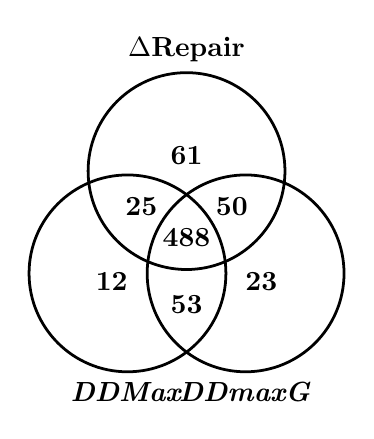
\begin{tikzpicture}[circ/.style={draw=black,line width=1pt,fill=none,shape=circle,minimum width=2.5cm,minimum height=2.5cm},lbl/.style={font=\bfseries}]
        \node[draw=none,minimum width=1.5cm,minimum height=1.29904cm,inner sep=0,outer sep=0] at (0,0) (anchor) {};
        \node[circ] at (anchor.south west) (g1) {};
        \node[circ] at (anchor.south east) (g2) {};
        \node[circ] at (anchor.north) (g3) {};
        \node[lbl,anchor=north] at (g1.south) {\ddmax};
        \node[lbl,anchor=north] at (g2.south) {\ddmaxg};
        \node[lbl,anchor=south] at (g3.north) {\drepair};
        \node[lbl] at ($(g1)!0.5!(g2) - (0,.4)$) {53};
        \node[lbl] at ($(g2)!0.5!(g3) + (.2,.2)$) {50};
        \node[lbl] at ($(g1)!0.5!(g3) + (-.2,.2)$) {25};
        \node[lbl] at ($(anchor.center) - (0,.2)$) {488};
        \node[lbl] at ($(g1.center) - (.2,.1)$) {12};
        \node[lbl] at ($(g2.center) - (-.2,.1)$) {23};
        \node[lbl] at ($(g3.center) + (0,.2)$) {61};
    \end{tikzpicture}
\end{minipage}
\vspace{-0.4cm}
\label{fig:repair-complementarity}
\end{figure}


\begin{result}
\approach %outperforms and 
is complementary to the state-of-the-art methods (lexical and syntactic \ddmax). 
It %is the only technique that can 
solely completes 9\% of all repairs, which is 
up to five times 
as much as \ddmax.
\end{result}











\subsection{RQ3 Efficiency} %\todo{fix to new evaluation results}
Let us evaluate the time performance of our approach.
For a balanced evaluation, we
analyse a set of 480 invalid inputs % files
that were completely repaired by all three approaches within %, in less than
the four minutes timeout, %. % (120,000ms).
without %accounting for
data collection and % or 
experimental
analysis time.
\Cref{tab:efficiency} %and figure X}
reports the efficiency of all three approaches. % approach compared to ddmax. %the state-of-the-art methods.


\textit{\approach is considerably efficient in input repair: It is reasonably fast, it takes about 10 seconds to repair an invalid input, on average}. However, it is about five times slower than \ddmax (two to three seconds, on average). 
\Cref{tab:efficiency} %} %  and Table/Figure X show}
shows %the %Inspecting
that the execution time
of \approach %syntactic ddmax
is much higher %lower
than that of syntactic and lexical \ddmax. 
This result is %ese findings are
due to the %can be explained
number of program runs required by \approach, especially due to its additional repair operation (input synthesis) and its extra oracle checks (incompleteness and parse-boundary).
\approach is reasonably efficient, similar to \ddmax, the number of program runs 
is its main performance bottleneck. %of \approach.  % as well as \ddmax. %all three approaches. % to the

\begin{result}
\approach is reasonably fast (10 seconds), but it 
is 5$\times$ slower than \ddmax because it requires
additional operations and oracle checks. 
\end{result}

\begin{table}[!tbp]\centering
\caption{Efficiency of \approach vs. \ddmax, lowest runtime and smaller number of program runs %and significant \% improvement in efficiency
are in \textbf{bold}. %, second-best time performance is in \textit{italics}
}
\begin{tabular}{|l |  r  r | r  r |}
\hline
&  \multicolumn{2}{c|}{\textbf{Runtime (s)}} & \multicolumn{2}{c|}{\textbf{\#Prog. Runs}}  \\
\textbf{Techniques} %& \textbf{Inputs}
&  \textbf{Avg.}  & \textbf{Total} & \textbf{Avg.}  & \textbf{Total} \\
\hline
\textbf{Lex. \ddmax} & 3.4 & 1653 & 3260 & 1564781 \\
\textbf{Syn. \ddmax} & \textbf{2.0} & \textbf{982}  & \textbf{2075}  & \textbf{995802}  \\
\hline
\textbf{\approach} &  10.2 & 4938  & 11537 & 5537601  \\
\hline
\end{tabular}
\label{tab:efficiency}
\end{table}

\subsection{RQ4 Perfect Repair.}
\revise{In this research question, we would like to evaluate the number of files that have been repaired perfectly by each approach, that is - the repaired file is exactly the same file as the file before it was mutated.
Since this obviously limits the number of files we can use in the evaluation to the artificially mutated files, the total number of files is smaller in this section of the experiments.}

\revise{We report the number of repaired files in \cref{tab:perfectrepairs}.
The total number of perfectly repaired files for \approach (49) is (17\%) higher than for \ddmax (42), while \ddmaxg did not manage to perfectly repair any file at all. We attribute this 
%This might be due 
to the fact that \ddmaxg needs to parse and un-parse all input files to work on the parse tree instead of the characters, which introduces noise, e.g.,  by changing whitespaces and line breaks in the files.
}

\revise{
We also inspect the files that were repaired solely by \approach, \ddmax 
% \textit{only}
or both 
%, as well as the 
%If we take a look at the 
%overlap of files that could be perfectly repaired  by both 
approaches (\cref{fig:perfectlyrepairedvenndiagram}).  We found that 
\approach \textit{solely} repaired 
twice (2.17$\times$) as many input files
as 
% in comparison to 
\ddmax: 
\autoref{fig:perfectlyrepairedvenndiagram} shows that 
13 input files were perfectly repaired by \approach  \textit{solely},  in comparison to six (6) input files for \ddmax  \textit{solely}. 
Meanwhile,  36 input files were perfectly repaired by both methods. 
Overall,  these results showcase the ability of \approach to repair files that are difficult to repair for \ddmax.
}

\begin{result}
\approach completed (17\%) more perfect repairs than \ddmax. It solely completed twice (2$\times$) as many perfect repairs 
%exclusively 
%in comparison to 
as \ddmax (13 vs.  6 perfect repairs). 
%:
%While \approach completed 13 repairs, 
\end{result}

\begin{table}[!tbp]\centering
\caption{Number of \textit{perfectly} repaired files for \approach in comparison to \ddmax and \ddmaxg
}
%\begin{tabular}{|l |  r  r  r  r | r |}
\begin{tabular}{|p{4.0cm}|p{1.5cm}|p{1.5cm}|p{1.5cm}|p{1.5cm}|p{1.5cm}|}
\hline
\textbf{Techniques}&  \textbf{INI}&\textbf{cJSON} &\textbf{sExp}&\textbf{TinyC}&\textbf{Total}  \\
\hline
\textbf{Lex. \ddmax}  & 1 & 14 & 2 & 25 & 42 \\
\textbf{Syn. \ddmaxg} & 0 & 0  & 0 & 0  & 0  \\
\hline
\textbf{\approach} &  1 & 18  & 0 & 30 & 49  \\
\hline
\end{tabular}
\label{tab:perfectrepairs}
\end{table}

\begin{figure}[!tbp]\centering
\caption{\centering Venn Diagram showing the 
%overlap of 
files that were \textit{perfectly} repaired (\textit{solely}) by \approach,  \ddmax or both approaches. 
}
\centering
\begin{minipage}[b]{0.45\textwidth}
    \centering
    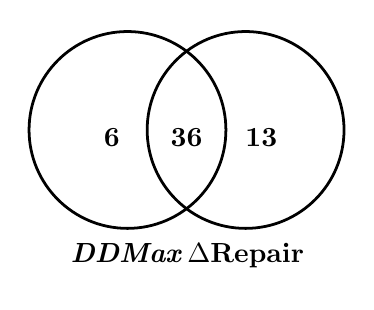
\begin{tikzpicture}[circ/.style={draw=black,line width=1pt,fill=none,shape=circle,minimum width=2.0cm,minimum height=2.5cm},lbl/.style={font=\bfseries}]
        \node[draw=none,minimum width=1.5cm,minimum height=1.29904cm,inner sep=0,outer sep=0] at (0,0) (anchor) {};
        \node[circ] at (anchor.south west) (g1) {};
        \node[circ] at (anchor.south east) (g2) {};
        \node[lbl,anchor=north] at (g1.south) {\strut\ddmax};
        \node[lbl,anchor=north] at (g2.south) {\strut\approach};
        \node[lbl] at ($(g1)!0.5!(g2) - (0,.1)$) {36};
        \node[lbl] at ($(g1.center) - (.2,.1)$) {6};
        \node[lbl] at ($(g2.center) - (-.2,.1)$) {13};
    \end{tikzpicture}
\end{minipage}
\vspace{-0.4cm}
\label{fig:perfectlyrepairedvenndiagram}
\end{figure}
%\end{comment}

%\subsection{RQ5 Quality of Repaired Files}
%\todo{EZ: Write RQ5}

\section{Threats to Validity}
\label{sec:threats}

%\todo{EZ: Add Rich Feedback Oracle problem to threats (the approach very much relies on reliable oracles and even one small faulty feedback might make the whole input unrepairable)}

\subsection{External Validity} This refers to the \textit{generalizability} of our approach, i.e., 
the threat that \approach may not generalize to other programs and input formats. 
To mitigate this threat, we have employed four well-known input formats with varying complexity, their corresponding programs also have  varying sizes (375 to 3062 LOC) and maturity (6 to 21 years old). 


\subsection{Internal Validity} This concerns the \textit{correctness} of our implementation and evaluation, especially if we have correctly implemented \approach and the baselines. We mitigate this threat by testing our implementation of all approaches on small and simple test inputs to ensure the they behave as described. 


\subsection{Construct Validity} This concerns the test oracle and parse-failure feedback employed in our evaluation. To ensure all subjects provide the expected \textit{incomplete} and \textit{(in)correct} feedback, we tested the programs on sample invalid inputs and modified the subject program, if needed. 


\section{Limitations}
Our approach (\approach) and empirical evaluations may be limited by the following: % validity threats:

\subsection{Limited to Data Repair} The repair produced by our approach aim to ensure maximal data recovery, but it does not ensure that the intended user information is preserved. Hence, \approach is limited to repair of the input data, but not the intended information. 


\subsection{Input Constraints and Semantics} \approach does not address concerns about recovering or preserving the input constraints or intended semantics of the input data. For instance, repairing an invalid checksum or hash requires such information, and \approach will be limited for this use cases. However, it would provide repair-candidates that allow end-users to debug such semantic issues. 
\revise{
In addition, inputs with significant semantic corruption may not be effectively repaired by \drepair. Even though \drepair is effective in fixing structural parts of invalid inputs, when the corruption is in the semantic part, the missing data becomes difficult to recover. Examples include corrupted numbers in calculations, and dates.}


\subsection{Repair via Input Synthesis} 
\revise{Firstly, the repair via synthesis approach of \approach is exhaustive, thus it can quickly become computationally expensive.} 
Secondly, the repair via synthesis operation %(i.e., insertion) % operation) 
of our approach poses the risk of introducing input elements with unintended semantic consequences. 
Specifically, insertion operations may lead %cause further 
to data corruption and information distortion. To mitigate this threat, \approach provides several valid candidate repairs ranked by the edit distance 
of each repair-candidate from the original input. %to %.
Hence, we 
encourage end-users to select the best semantically-fit repair from the 
potential repair-candidates provided by \approach. 


\done{Do you talk about the risk of input synthesis (which may be perceived as greater than the risk of input deletion) somewhere? A small lexical change may have large semantical consequences -- AZ}






\section{Related Work}
\label{sec:relatedwork}

Let us discuss the state-of-the-art input repair approaches and how they compare to \approach. 

\subsection{Black-box Input Repair} 
A few techniques have been proposed to analyze input data without program analysis, albeit with the aim of understanding and localizing faults in the program. The earliest works were either focused on simplifying failure-inducing inputs~\cite{zeller2002simplifying, clause2009penumbra}, or isolating fault-revealing input fragments~\cite{hierarchicalDD, sterling2007automated}. Notably, the minimizing delta debugging algorithm (\ddmin) is focused on reducing failure-inducing inputs in order to diagnose and localize faults in the program. More recently, Kirschner et al.~\cite{kirschner2020debugging} proposed a maximizing variant of the delta debugging algorithm (\ddmax) to repair invalid inputs to subsets via deletion, we compare \approach to \ddmax in this work. In contrast to \ddmax, \approach also synthesizes input elements to complete input repair. 


\subsection{White and Grey-box Input Repair} Some techniques employ program analysis to fix invalid inputs. As an example, \emph{docovery}~\cite{docovery:ase14} applies symbolic execution to change broken inputs to take error-free paths in the subject program. Similarly, Ammann and Knight~\cite{data_diversity} proposed a method to transform invalid inputs into valid inputs by analyzing the region of the input causing the fault and changing those regions to avoid the fault. Unlike these methods, \approach 
is black-box, it relies on the parse-failure feedback of the subject program. 


\subsection{Constraint-based Input Repair} %via Constraint Learning:} 
These approaches automatically learn input constraints then enforce the learned constraints to repair invalid inputs~\cite{hussain2010dynamic, Demsky:2006:IED:1146238.1146266} 
These constraints are often extracted from valid inputs~\cite{Long:2012:AIR:2337223.2337233, Rinard:2007:LCZ:1297027.1297072}, specified with predicates~\cite{elkarablieh2008juzi}, model-based systems~\cite{Demsky:2003:ADR:949343.949314}, goal-directed reasoning~\cite{1553560}, dynamic symbolic execution~\cite{hussain2010dynamic} or invariants~\cite{Demsky:2006:IED:1146238.1146266}. For instance, \emph{S-DAGs}~\cite{scheffczyk2004s} enforce constraints on invalid inputs in a semi-automatic way. Unlike these approaches, \approach does not learn input constraints, it employs input synthesis and parse-failure feedback to fix invalid inputs. 


\subsection{Parser-directed Input Repair} %:}
This refers to the input repair schemes of parsers, interpreters and compilers~\cite{parr2011ll, diekmann2020dont, aho1972minimum, hammond1984survey, backhouse1979syntax}. 
These techniques employ operations such as insertion, deletion and replacement of symbols~\cite{anderson1981locally, cerecke2003locally, anderson1983assessment}, extending forward or backwards from a parser error~\cite{burke1982practical, mauney1982forward}, or more general methods of recovery and diagnosis~\cite{krawczyk1980error, aho1972minimum}. 
In this work, we compare \approach to the recovery scheme of the ANTLR parser generator~\cite{parr2011ll} which leverages the input grammar to guide input repair. %Compared to \approach, t
Unlike \approach which aims to fix an invalid input, these schemes need an input grammar, and aim to ensure the compiler does not halt while parsing. 





\section{Conclusion}
\label{sec:conclusion}
This paper presents \approach, an input repair approach that employs input synthesis and parse-failure feedback (i.e., incomplete and (in)correct checks) to repair invalid inputs. 
%Our approach is black-box, does not require program analysis or an input grammar. 
We evaluate the data recovery, repair effectiveness, and efficiency of our approach, in comparison to the state-of-the-art methods. We show that \approach has a very high data recovery rate, it recovered 91\% of input data. 
It is also very effective and efficient in input repair---it completes the repair of about four in five invalid inputs (77\%) within four minutes. Furthermore, we demonstrate that our approach is up to 35\% more effective than the best 
best baseline---(syntactic) \ddmax, without using an input grammar. In summary, this work demonstrates that combining parse-failure feedback and input synthesis are important for the effective repair of invalid inputs, especially in the absence of an input specification 
and program analysis.
In the future, we plan to investigate how to improve the performance of our approach by learning input semantics and constraints.

We provide our implementation, experimental data and results for easy replication, scrutiny and reuse:


 \begin{center}
   \textbf{anonymous} %\url{https://tinyurl.com/fsynth}}
 \end{center}







\bibliographystyle{ACM-Reference-Format}
\bibliography{tosem23-brepair}






\end{document}
\endinput
\bibliographystyle{ACM-Reference-Format}
\bibliography{fse2025-drepair}

\end{document}
\endinput
%%
%% End of file `sample-acmsmall-conf.tex'.
